%&tfgheader

\documentclass[
  a4paper,
  12pt,
  spanish,
  dvipsnames,
  footinclude,
  headinclude,
  %oneside,
]{scrbook}

\usepackage{expl3}
\usepackage{xparse}

%-------------------------------------------------------------------------------
%	ENTORNOS MATEMÁTICOS
%-------------------------------------------------------------------------------

\usepackage{amsmath, amsthm, amssymb}

\newtheoremstyle{theorem-style}  % Nombre del estilo
{\topsep}                                  % Espacio por encima
{\topsep}                                  % Espacio por debajo
{\itshape}                                  % Fuente del cuerpo
{0pt}                                  % Identación
{\scshape}                      % Fuente para la cabecera
{}                                 % Puntuación tras la cabecera
{5pt plus 1pt minus 1pt}                              % Espacio tras la cabecera
{\lsc{{\thmname{#1}\thmnumber{ #2}}.\thmnote{ (#3.)}}}  % Especificación de la cabecera
\theoremstyle{theorem-style}
\newtheorem{theorem}{Teorema}[section]
\newtheorem{corollary}[theorem]{Corolario}
\newtheorem{lemma}[theorem]{Lema}
\newtheorem{proposition}[theorem]{Proposición}
\newtheorem{question}{Pregunta}
\newtheorem{conjecture}[theorem]{Conjetura}
\newtheorem{remark}[theorem]{Nota}
\newtheoremstyle{definition-style}  % Nombre del estilo
{\topsep}                                  % Espacio por encima
{\topsep}                                  % Espacio por debajo
{}                                  % Fuente del cuerpo
{0pt}                                  % Identación
{}                      % Fuente para la cabecera
{.}                                 % Puntuación tras la cabecera
{5pt plus 1pt minus 1pt}                              % Espacio tras la cabecera
{\lsc{{\thmname{#1}\thmnumber{ #2}}\thmnote{ (#3)}}}  % Especificación de la cabecera
\theoremstyle{definition-style}
\newtheorem{definition}[theorem]{Definición}
\newtheorem{example}[theorem]{Ejemplo}
\newtheorem{notation}[theorem]{Notación}
\newtheorem{exercise}[theorem]{Ejercicio}

% Matemáticas

\usepackage{mathtools}
\usepackage{commath}

% Enlaces y colores

\usepackage{hyperref}
\usepackage{xcolor}
\hypersetup{
  colorlinks=true,
  citecolor=,
}

% Otros elementos de página

\usepackage{enumitem}
\setlist[itemize]{ noitemsep, leftmargin=*}
\setlist[enumerate]{noitemsep, leftmargin=*}

\DeclareRobustCommand{\textacr}[1]{\textls{\small #1}}

% Código

\usepackage{listings}
\lstset{
	basicstyle=\ttfamily,%
	breaklines=true,%
	captionpos=b,                    % sets the caption-position to bottom
  tabsize=2,	                   % sets default tabsize to 2 spaces
  frame=none,
  numbers=left,
  xleftmargin=18pt,
  stepnumber=1,
  aboveskip=12pt,
  showstringspaces=false,
  keywordstyle=\bfseries,
  commentstyle=\itshape,
  numberstyle=\scriptsize\bfseries
}
\renewcommand{\lstlistingname}{Listado}

%\endofdump

%-------------------------------------------------------------------------------
%	PAQUETES
%-------------------------------------------------------------------------------

% Idioma

\usepackage[es-noindentfirst, es-lcroman, es-tabla]{babel}
\spanishdashitems

% Citas de texto en línea/bloque

\usepackage[autostyle]{csquotes}

% Tikz

\usepackage{tikz}
\usetikzlibrary{babel}
\usepackage{float}

% Bibliografía

\usepackage[sorting=none, style=apa, isbn=true]{biblatex}
\addbibresource{bibliografia.bib}

% Lorem ipsum

\usepackage{blindtext}

% Algoritmos

\usepackage[linesnumbered, onelanguage, ruled]{algorithm2e}
\SetAlCapFnt{\sffamily}
\SetAlCapNameFnt{\sffamily}
\newcommand\mycommentfont[1]{\sffamily\textcolor{darkgray}{#1}}
\SetCommentSty{mycommentfont}
%\SetAlFnt{\sffamily}
%\SetKwSty{sffamily}
\SetAlCapSkip{.5em}
\SetAlgoCaptionLayout{raggedright}
\SetAlgorithmName{Algoritmo}{Algoritmo}{Lista de algoritmos}
%\SetAlgoSkip{medskip}
\SetAlgoInsideSkip{medskip}

% Entorno algoritmo con líneas pero caption debajo
\makeatletter
\newenvironment{Ualgorithm}[1][htpb]{\def\@algocf@post@ruled{\color{gray}\hrule  height\algoheightrule\kern6pt\relax}%
\def\@algocf@capt@ruled{under}%
\setlength\algotitleheightrule{0pt}%
\SetAlgoCaptionLayout{raggedright}%
\begin{algorithm}[#1]}
{\end{algorithm}}
\makeatother

\makeatletter
\newcommand{\setalgotoprulecolor}[1]{\colorlet{toprulecolor}{#1}}
\let\old@algocf@pre@ruled\@algocf@pre@ruled % Adjust top rule colour
\renewcommand{\@algocf@pre@ruled}{\textcolor{toprulecolor}{\old@algocf@pre@ruled}}

\newcommand{\setalgobotrulecolor}[1]{\colorlet{bottomrulecolor}{#1}}
\let\old@algocf@post@ruled\@algocf@post@ruled % Adjust middle rule colour
\renewcommand{\@algocf@post@ruled}{\textcolor{bottomrulecolor}{\old@algocf@post@ruled}}

\newcommand{\setalgomidrulecolor}[1]{\colorlet{midrulecolor}{#1}}
\renewcommand{\algocf@caption@ruled}{%
  \box\algocf@capbox{\color{midrulecolor}\kern\interspacetitleruled\hrule
    width\algocf@ruledwidth height\algotitleheightrule depth0pt\kern\interspacealgoruled}}
\makeatother

\setalgotoprulecolor{gray}
\setalgomidrulecolor{gray}
\setalgobotrulecolor{gray}

%-------------------------------------------------------------------------------
%	NOTSOCLASSICTHESIS & FUENTES
%-------------------------------------------------------------------------------

\usepackage[
  drafting=true,
  %tocaligned=true,
  dottedtoc=true,
  parts,
  floatperchapter,
  pdfspacing,
  beramono=false,
  palatino=false,
]{notsoclassicthesis}

\setmainfont[%
Contextuals=Alternate,
SmallCapsFeatures={LetterSpace=1}]%
{EBGaramond}
\setsansfont[Scale=0.8]{Open Sans} 
\renewfontface\chapterNumber[Scale=7, Color=000000]{EBGaramond}
\setmonofont[Scale=0.75]{Go Mono}

\usepackage[math-style=TeX, bold-style=ISO]{unicode-math}
\setmathfont{Garamond Math}[StylisticSet={3}]

\usepackage{caption}
\captionsetup{font=sf, labelfont=bf, justification=raggedright,singlelinecheck=false}

\linespread{1.1}
\setlength{\parindent}{1.5em}

% Operadores

\let\deg\relax
\DeclareMathOperator{\deg}{gr}
\DeclareMathOperator{\lc}{cl}

%-------------------------------------------------------------------------------
%	TÍTULO
%-------------------------------------------------------------------------------

\title{Algoritmo de Peterson-Gorenstein-Zierler para códigos cíclicos sesgados}
\renewcommand{\myVersion}{0.6} 

\author{José María Martín Luque}

\date{\normalsize\today}

% Portada

\usepackage{eso-pic}
\newcommand\BackgroundPic{%
	\put(0,0){%
		\parbox[b][\paperheight]{\paperwidth}{%
			\vfill
			\centering
      % Indicar la imagen de fondo en el siguiente comando
			
\includegraphics[width=\paperwidth,height=\paperheight,%
			keepaspectratio]{assets/portada-ugr-color}%
			\vfill
    }
  }
}

%-------------------------------------------------------------------------------
%	CONTENIDO
%-------------------------------------------------------------------------------

%\includeonly{teoria-codigos}

\begin{document}

%\maketitle

\begin{titlepage}
  \AddToShipoutPicture*{\BackgroundPic}
  \phantomsection
  \pdfbookmark[1]{Title}{title}

  % Para que el título esté centrado en la página.
  % Los valores numéricos deberán elegirse de acuerdo con el diseño de
  % página (sobre todo si se cambia la opción BCOR o DIV).
  \begin{addmargin}[2.05cm]{0cm}
  \begin{flushleft}
    \Large
    \hfill\vfil

    \vfill\vfill

    \textsf{Facultad de Ciencias}\\[.5em]
    \textsf{E.T.S. de Ingenierías Informática y de Telecomunicación} \\
    \vfill\vfill

    \textsf{\Large Doble Grado en Ingeniería Informática y Matemáticas} \vfill


    %\textsc{trabajo de fin de grado}
    \spacedlowsmallcaps{Trabajo de Fin de Grado}

    \begingroup
    \Huge{Algoritmo de Peterson-Gorenstein-Zierler para códigos cíclicos sesgados} \\ \bigskip
    \endgroup

    [\,\today\ a las \thistime\ -- \myVersion\,]

    \vfill\vfill\vfill\vfill

    \textsf{\normalsize{Presentado por}}\\[6pt]
    {\huge\textrm{José María Martín Luque}}

    \vspace*{0.7cm}

    \textsf{\normalsize{Tutorizado por}}\\[6pt]
    {\huge\textrm{Gabriel Navarro Garulo}}

    \vfill
    \textsf{Curso académico 2019--2020}
  \end{flushleft}
  \end{addmargin}

\end{titlepage}

\newpage

\chapter*{Resumen}

Resumen.

\chapter*{Summary}

Summary.

{\hypersetup{hidelinks}
\tableofcontents
}

\newpage

\chapter*{Introducción}
 
El artículo de Claude Shannon \textit{Mathematical Theory of Cryptography} \parencite{shannon_mathematical_1945} y su ampliación posterior, \textit{Mathematical Theory of Communication} \parencite{shannon_mathematical_1948} dieron a luz a dos disciplinas hoy plenamente establecidas: la teoría de información y la teoría de códigos.
El objetivo principal de estas disciplinas es el de establecer mecanismos de comunicación que sean \emph{eficientes} y \emph{fiables} en ambientes posiblemente hostiles.
La eficiencia requiere que la transmisión de la información no necesite de demasiados recursos, sean materiales o temporales.
Por otro lado, la fiabilidad requiere que el mensaje recibido en una comunicación sea lo más parecido posible, dentro de unos márgenes de tolerancia, al mensaje original.
La teoría de la información se encarga del estudio tanto de la representación de la información como de la capacidad que tienen los sistemas para transmitir y procesar la información. 
Por otra parte, la teoría de códigos se basa en los resultados de la teoría de la información para el diseño y desarrollo de modelos de transmisión de información mediante herramientas algebraicas.

A pesar de que digamos que Shannon fue el padre de estas disciplinas, el problema de codificar la información no surge, ni mucho menos, entonces.
De hecho, el filósofo inglés Francis Bacon ya afirmó en el año 1623 que únicamente son necesarios dos símbolos para codificar toda la comunicación.
\blockquote[{\cite[30]{dyson_catedral_2015}}]{La transposición de dos letras en cinco emplazamientos bastará para dar 32 diferencias [y] por este arte se abre un camino por el que un hombre puede expresar y señalar las intenciones de su mente, a un lugar situado a cualquier distancia, mediante objetos ... capaces solo de una doble diferencia.}
Efectivamente, hoy en día la codificación binaria forma parte de prácticamente todos los aspectos nuestras vidas.

Sin embargo, el problema más relevante —y el que nos ocupa— es el de codificar la información para que se produzca una correcta transmisión y recepción de los mensajes a través de un canal.
Como parte de su teoría Shannon introdujo lo que posteriormente se conocería como \emph{modelo de comunicación de Shannon}, un esquema simplificado de cómo se produce la transmisión de información entre emisor y receptor a través de un canal.
\begin{figure}
  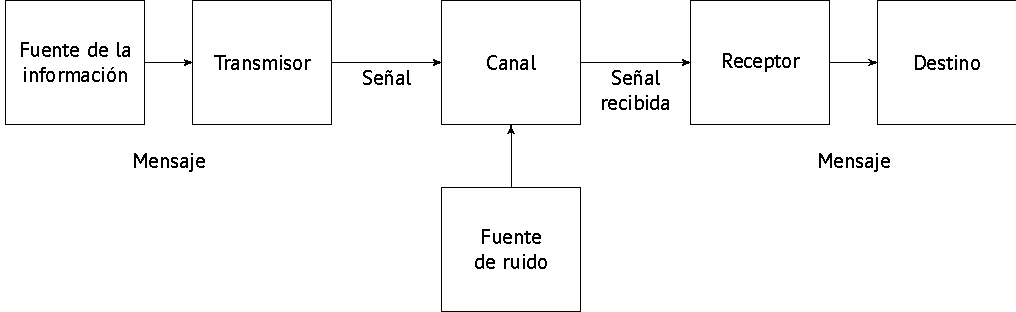
\includegraphics[width=\textwidth]{assets/shannon-communication-model.pdf}
  \caption*{Modelo de comunicación de Shannon}
\end{figure}
Al enviar la información a través del canal es posible que, debido al ruido que pueda haber en el mismo, se produzcan interferencias que alteren el mensaje enviado.
Por supuesto recibir un mensaje alterado no es deseable, pues es posible que la alteración sea tal que el mensaje recibido sea ilegible.
La teoría de códigos trata por tanto de diseñar estructuras algebraicas que permitan la corrección de errores por parte del receptor del mensaje.
Estas estructuras son los códigos, y son el objeto matemático sobre el que orbita todo este trabajo.

\section*{Enfoque}

El título de este trabajo es «Algoritmo de Peterson-Gorenstein-Zierler para códigos cíclicos sesgados», y como tal, expresa el objetivo último del mismo: exponer y estudiar este algoritmo.
En consecuencia, dirigiremos nuestra atención a los conceptos y herramientas necesarios para ello.
En cuanto a los fundamentos matemáticos necesarios, hablaremos de cuerpos finitos, anillos de polinomios sobre cuerpos finitos y anillos de polinomios de Ore sobre cuerpos finitos.
La teoría de códigos explicada se centrará en la exposición de los códigos lineales y de los códigos cíclicos, así como de las familias de códigos concretas sobre las que trabajarán los algoritmos que vamos a describir.
Para comprender mejor el citado algoritmo estudiaremos también la versión original, de mitad del siglo pasado, para los conocidos como códigos BCH.
A lo largo del trabajo ilustraremos algunos ejemplos con el sistema algebraico computacional SageMath \parencite{the_sage_developers_sagemath_2020}.

\section*{Motivación}

Los códigos cíclicos son muy utilizados porque son muy sencillos de implementar en sistemas digitales utilizando lo que se conoce como registros de desplazamiento, que permiten realizar desplazamientos de bits fácilmente.
El algoritmo Peterson-Gorenstein-Zierler para códigos BCH es interesante porque es uno de los primeros algoritmos eficientes que se desarrollaron para códigos cíclicos.
El uso de anillos de polinomios de Ore nos permite obtener una mayor cantidad de códigos cíclicos sesgados, simplemente variando el automorfismo utilizado.
Esta gran variedad permite encontrar códigos que tengan propiedades interesantes que mejoren a las familias de códigos cíclicos conocidas.
Finalmente, el algoritmo de Peterson-Gorenstein-Zierler para códigos cíclicos sesgados que se expone permite decodificarlos con una eficiencia igual o superior a la que presenta el algoritmo clásico para códigos BCH.

\section*{Objetivos}

Los objetivos de este trabajo son los siguientes. \begin{itemize}
  \item Estudio de las nociones básicas sobre Teoría de Códigos lineales.
  \item Estudio de las extensiones de Ore y de sus cocientes.
  \item Exponer el algoritmo de Peterson-Gorenstein-Zierler para códigos cíclicos sesgados.
  \item Implementación de sistemas de decodificación en Python usando SageMath.
\end{itemize}

\section*{Esquema}

En los tres primeros capítulos introduciremos todos los fundamentos matemáticos necesarios, así como las definiciones y propiedades fundamentales de los códigos lineales y de los códigos cíclicos.
El capítulo cuarto ahondaremos en la familia de los códigos BCH y presentaremos el algoritmo original de Peterson-Gorenstein-Zierler para esta familia de códigos.
En el capítulo quinto explicamos las estructuras matemáticas que constituyen la base de los códigos cíclicos sesgados, los anillos de polinomios de Ore, para ya introducirlos propiamente en el capítulo sexto.
Finalmente, en el capítulo séptimo describimos el funcionamiento del algoritmo de Peterson-Gorenstein-Zierler para códigos cíclicos sesgados.





\chapter{Preliminares}

En este capítulo se detallan algunos conceptos básicos de Álgebra que son necesarios para la comprensión más adelante de la teoría de códigos. Según \parencite{cohn_algebra_1982} y \parencite{cohn_algebra_1989}.

\section{Monoides}

\begin{definition}
  Un \textit{monoide} es un conjunto \(S\) con un elemento \(e\) y una aplicación \(\mu: S^2 \to S\) tal que si \(\mu(x, y)\) es el resultado de aplicar \(\mu\) a la pareja de elementos \(x, y \in S\), se verifican: \begin{enumerate}
    \item \(\mu(x, \mu(y, z)) = \mu(\mu(x, y), z)\) para todo \(x, y, z \in S\).
    \item \(\mu(e, x) = \mu(x, e) = x\) para todo \(x \in S\).
  \end{enumerate}
\end{definition}

Obsérvese que, por definición, un monoide siempre tiene al menos un elemento. A la aplicación \(\mu\) que actúa sobre parejas de elementos se le llama \textit{operación binaria} y al elemento \(e\), elemento neutro de \(\mu\).

\section{Anillos}

\begin{definition}
  Un \textit{anillo}.
\end{definition}
\chapter{Fundamentos de teoría de códigos}

En la introducción ya hemos visto cuáles son los objetivos de la teoría de códigos, así como el medio principal del que se sirve: el álgebra.
Esta sección vamos a comentar algunos de los conceptos y resultados fundamentales de la teoría de códigos.
Daremos la definición más sencilla de código para posteriormente estudiar otras estructuras más complejas, los códigos lineales y los códigos cíclicos, así como resultados básicos asociados a ellos.
Finalmente, estudiaremos la versión original del algoritmo de Peterson-Gorenstein-Zierler, diseñado para un tipo de códigos, los \textacr{BCH}.

Las definiciones y los resultados comentados en esta sección seguirán lo descrito en \parencite[cap. 1, 3-5]{huffman_fundamentals_2003} y \parencite{podesta_introduccion_2006}.

\section{Códigos lineales}

Vamos a comenzar nuestro estudio con los códigos lineales, pues son los más sencillos de comprender. 
Consideremos el espacio vectorial de todas las \(n\)-tuplas sobre el cuerpo finito \(\mathbb F_q\), al que denotaremos en lo que sigue como \(\mathbb F_q^n\). 
A los elementos \((a_1, \dots, a_n)\) de \(\mathbb F_q^n\) los notaremos usualmente como \(a_1\!\cdots a_n\).

\begin{definition}
  Un \((n, M)\) \textit{código} \(\mathcal C\) sobre el cuerpo \(\mathbb F_q\) es un subconjunto de \(\mathbb F_q^n\) de tamaño \(M\). 
  Si no hay riesgo de confusión lo denotaremos simplemente por \(\mathcal C\). 
  A los elementos de \(\mathcal C\) los llamaremos \textit{palabras codificadas}, \textit{palabras código} o \textit{codewords} en inglés.
  A \(n\) se le llama \(longitud\) del código.
\end{definition}

Por ejemplo, un \((5,4)\) código sobre \(\mathbb F_2\) puede ser el formado por los siguientes elementos: \[
  10101,\qquad
  10010,\qquad
  01110,\qquad
  11111.
\]
Como se puede ver realmente un código es un objeto muy sencillo.
Concluimos que es necesario añadir más estructura a los códigos para que puedan ser de utilidad.
Esto motiva la siguiente definición.

% TODO: Ejemplo de un código que no es lineal
% Quizás que ilustre por qué es necesario añadirles más estructura

\begin{definition}
  Decimos que un código \(\mathcal C\) es un código \textit{lineal de longitud \(n\) y dimensión \(k\)} —abreviado como \([n, k]\)-\textit{lineal}, o como \([n, k]_q\)~-\textit{lineal} en caso de querer informar del cuerpo base— si dicho código es un subespacio vectorial de \(\mathbb F_q^n\) de dimensión \(k\).
\end{definition}

% TODO: Gabriel me comenta que ponga punto y seguido, aunque no sé si se refiere

\begin{remark}
  Un código lineal \(\mathcal C\) tiene \(q^k\) palabras codificadas.
\end{remark}

Así, hemos pasado de trabajar con un objeto que no tiene estructura alguna a trabajar con espacios vectoriales, cuyas propiedades son conocidas y disponemos de numerosas herramientas para tratarlos.
Un primer ejemplo es la siguiente definición.

\begin{definition}
  Una \textit{matriz generadora} para un \([n, k]\) código \(\mathcal C\) es una matriz \(k \times n\) cuyas filas conforman una base de \(\mathcal C\).
\end{definition}

\begin{definition}
  Para cada conjunto \(k\) de columnas independientes de una matriz generadora \(G\) el conjunto de coordenadas correspondiente se denomina \textit{conjunto de información} para un código \(\mathcal C\). 
  Las \(r = n - k\) coordenadas restantes se llaman \textit{conjunto redundante}, y el número \(r\), la \textit{redundancia} de \(\mathcal C\).
\end{definition}

Si las primeras \(k\) coordenadas forman un conjunto de información el código tiene una única matriz generadora de la forma \([I_k \mid A]\), donde \(I_k\) es la matriz identidad \(k \times k\) y \(A\) es una matriz \(k \times r\). 
Esta matriz generadora se dice que está en \textit{forma estándar}.
A partir de cualquier matriz generadora siempre es posible obtener una matriz en forma estándar realizando una permutación adecuada de las coordenadas.
%Esta matriz resultante no será una matriz generadora del código inicial, pero sí de un código equivalente.

%Como un código lineal es el subespacio de un espacio vectorial, es el núcleo de una transformación lineal. En particular, existe una matriz \(H\) de dimensiones \(r \times n\), llamada \textit{matriz de comprobación de paridad} para un \([n, k]\) código \(\mathcal C\) definida por \begin{equation}
%  \mathcal C = \left\{x \in \mathbb F_q^n : H \mathbf x^T = 0 %\right\}.
%\end{equation}

Como un código lineal \(\mathcal C\) es un subespacio de un espacio vectorial, podemos calcular el ortogonal a dicho subespacio, obteniendo lo que llamaremos el \textit{código dual} (\textit{euclídeo}, si usamos el producto escalar usual) y que denotaremos por \(\mathcal C^{\perp}\).

\begin{definition}
  El \textit{código dual} \(\mathcal C^{\perp}\) de un código \(\mathcal C\) viene dado por \[\mathcal C^{\perp} = \left\{x \in \mathbb F_q^n : x \cdot c = 0 \quad \forall c \in \mathcal C\right\},\]
  donde \(\cdot\) representa el producto escalar usual.
\end{definition}

\begin{definition}
  Sea \(\mathcal C\) un \([n, k]\) código lineal. Una matriz \(H\) se dice que es \textit{matriz de paridad} si es una matriz generadora de \(\mathcal C^{\perp}\).
\end{definition}

\begin{proposition}
  Sea \(H\) la matriz de paridad de un \([n, k]\) código lineal \(\mathcal C\). 
  Entonces, \[\mathcal C = \left\{x \in \mathbb F_q^n : xH^T = 0\right\} = \left\{x \in F_q^n : Hx^T = 0\right\}.\]
\end{proposition}

\begin{proof}
  Sea \(c \in \mathcal C\) una palabra codificada. 
  Sabemos que la podemos expresar como \(c = uG\), donde \(u \in \mathbb F_q^k\) y \(G\) es una matriz generadora de \(\mathcal C\). 
  Tenemos entonces que \(c\cramped{H^T} = uG\cramped{H^T}\) y como \(G\cramped{H^T} = 0\) —por ser H matriz generadora del subespacio ortogonal \(\mathcal C\)— se tiene que \[\mathcal C \subset S_H = \left\{x \in \mathbb F_q^n : Hx^T = 0\right\},\] que es el espacio solución de un sistema de \(n - k\) ecuaciones con \(n\) incógnitas y de rango \(n - k\). Como \(\dim(S_H) = n - (n - k) = k = \dim L\), concluimos que \[L = S_H = \left\{x \in \mathbb F_q^n : Hx^T = 0\right\}.\qedhere\]
\end{proof}

Este último resultado, junto a la definición previa, nos conducen al siguiente teorema. 

\begin{theorem}
  Si \(G = [I_k \mid A]\) es una matriz generadora para un \([n, k]\) código \(\mathcal C\) en forma estándar entonces \(H = [-A \mid I_{n-k}]\) es una matriz de paridad para \(\mathcal C\).
\end{theorem}

Como nota final sobre nomenclatura de códigos duales, apuntamos que un código se dice \textit{autoortogonal} cuando \(\mathcal C \subseteq \mathcal C^{\perp}\), y \textit{autodual} cuando \(\mathcal C = \mathcal C^{\perp}\).

\subsection{Codificación y decodificación}

La forma estándar de codificar mensajes con códigos lineales es utilizando una matriz generadora.
Dado un mensaje \(\mathbf{m} \in \mathbb F_q^k\) podemos obtener la palabra codificada \(\mathbf{c}\) en \(\mathcal C\) realizando la operación \(\mathbf{c}= \mathbf{m}G\).
Vamos a verlo mejor con un ejemplo.

\begin{example}
  Sea \(\mathcal C\) \([3, 2]\) un código binario lineal y \(G\) la matriz generadora dada por 
  \[
    G = \begin{pmatrix}
      1 & 1 & 0 \\ 0 & 1 & 1
    \end{pmatrix} \in \mathcal M_{2 \times 3}(\mathbb F_2).
  \]
  Dado un mensaje \(\mathbf{m} = (x_1, x_2)\), se tiene que \[(x_1, x_2) \begin{pmatrix}
    1 & 1 & 0 \\ 0 & 1 & 1
  \end{pmatrix} = (x_1, x_1 + x_2, x_2),\] y por tanto esta matriz codifica de la forma \[00 \to 000, \quad 01 \to 011,\quad 10 \to 110,\quad 11 \to 101.\]
\end{example}

Observamos que una matriz generador \(G\) define una aplicación lineal de \(\mathbb F_q^k\) en \(\mathbb F_q^n\), de forma que el código obtenido es la imagen de dicha aplicación.
Podemos comprobar también que es posible codificar en los mismos códigos lineales utilizando distintas matrices generadores, lo que resultará en distintas palabras código para el mismo mensaje.
Veamos un ejemplo con el mismo código binario lineal que en el ejemplo anterior pero con distinta matriz generadora.

\begin{example}
  Sea \(\mathcal C\) \([3, 2]\) un código binario lineal y \(G\) la matriz generadora dada por 
  \[
    G = \begin{pmatrix}
      1 & 0 & 1 \\ 0 & 1 & 1
    \end{pmatrix} \in \mathcal M_{2 \times 3}(\mathbb F_2).
  \]
  Dado un mensaje \(\mathbf{m} = (x_1, x_2)\), se tiene que \[(x_1, x_2) \begin{pmatrix}
    1 & 0 & 1 \\ 0 & 1 & 1
  \end{pmatrix} = (x_1, x_2, x_1 + x_2),\] y por tanto esta matriz codifica de la forma \[00 \to 000, \quad 01 \to 011,\quad 10 \to 101,\quad 11 \to 110.\]
\end{example}

Observamos en este ejemplo que las primeras \(2\) coordenadas de cada palabra código son iguales a las del mensaje que las genera.
Pero en el código anterior también podemos encontrar el mensaje, lo que hay que fijarse en la primera y última coordenada.
Cuando un mensaje se encuentra incrustado íntegramente en la palabra código —aunque puede que desordenado— se dice que la codificación seguida es \textit{sistemática}.
En caso contario, se dice que es \textit{no-sistemática}.
Veamos un ejemplo de codificación no-sistemática con el mismo código binario lineal de antes.

\begin{example}
  Sea \(\mathcal C\) \([3, 2]\) un código binario lineal y \(G\) la matriz generadora dada por 
  \[
    G = \begin{pmatrix}
      1 & 0 & 1 \\ 1 & 1 & 1
    \end{pmatrix} \in \mathcal M_{2 \times 3}(\mathbb F_2).
  \]
  Dado un mensaje \(\mathbf{m} = (x_1, x_2)\), se tiene que \[(x_1, x_2) \begin{pmatrix}
    1 & 0 & 1 \\ 1 & 1 & 1
  \end{pmatrix} = (x_1 + x_2, x_2, x_1 + x_2),\] y por tanto esta matriz codifica de la forma \[00 \to 000, \quad 01 \to 111,\quad 10 \to 101,\quad 11 \to 010.\]
  Comprobamos que los mensajes \(01\) y \(11\) no están contenidos en las palabras código correspondientes, \(111\) y \(010\), respectivamente, luego la codificación es no-sistemática.
\end{example}

El proceso de decodificación de los mensajes es mucho más complicado, pues como se ha comentado hay que tener en cuenta las posibles interferencias que se hayan podido producir en la comunicación.
Los métodos de decodificación de códigos lineales en general se escapan del alcance de este trabajo, pues su objetivo principal es la descripción de un algoritmo de decodificación para un tipo concreto de códigos que veremos más adelante.

\subsection{Distancias y pesos}

% FIXME: revisar introducción

Códigos distintos poseen distintas propiedades, lo que implica que sus capacidades de corrección difieran.
En este apartado vamos a estudiar dos propiedades de los códigos 
muy relacionadas con esta idea.

\begin{definition}
  La \textit{distancia de Hamming} \(\operatorname{d}(\symbf{x}, \symbf{y})\) entre dos vectores \(\symbf{x}, \symbf{y} \in \mathbb F_q^n\) se define como el número de coordenadas en las que difieren \(\symbf{x}\) e \(\symbf{y}\).
\end{definition}

\begin{theorem}
  La función de distancia \(\operatorname{d}(\symbf{x}, \symbf{y})\) verifica las siguientes propiedades.
  \begin{enumerate}
    \item No negatividad: \(\operatorname{d}(\symbf{x}, \symbf{y}) \geq 0\) para todo \(\symbf{x}, \symbf{y}\in \mathbb F_q^n\).
    \item \(\operatorname{d}(\symbf{x}, \symbf{y}) = 0\) si y solo si \(\symbf{x} = \symbf{y}\).
    \item Simetría: \(\operatorname{d}(\symbf{x}, \symbf{y}) = \operatorname{d}(\symbf{y}, \symbf{x})\) para todo \(\symbf{x}, \symbf{y}\in \mathbb F_q^n\).
    \item Desigualdad triangular: \(\operatorname{d}(\symbf{x}, \symbf{z}) \leq \operatorname{d}(\symbf{x}, \symbf{y}) + \operatorname{d}(\symbf{y}, \symbf{z})\) para todo elemento \(\symbf{x}, \symbf{y}, \symbf{z}\in \mathbb F_q^n\).
  \end{enumerate}
\end{theorem}

\begin{proof}
  
\end{proof}

La \textit{distancia (mínima)} de un código \(\mathcal C\) es la menor distancia posible entre dos palabras codificadas distintas. 
Si la distancia mínima \(d\) de un \([n,k]\) código es conocida, nos referiremos a él como un \([n,k,d]\) código.
Este valor es importante pues nos ayuda a determinar la capacidad de corrección de errores del código \(\mathcal C\), como ilustra el siguiente teorema.

\begin{theorem}
  Sea \(\mathcal C\) un \([n, k, d]\) código. Entonces \(\mathcal C\) tiene capacidad de corrección de errores \[
    t = \left\lfloor \frac{d - 1}{2} \right\rfloor.
  \]
\end{theorem}

% MAYBE: hablar también de la capacidad de detección de errores? l = d - 1

Efectivamente, a mayor distancia mínima, mayor número de errores en el código se pueden corregir.
Otra medida interesante es el \textit{peso de Hamming}.

\begin{definition}
  El \textit{peso de Hamming} \(\operatorname{wt}(\symbf{x})\) de un vector \(\symbf{x}\) es el número de coordenadas distintas de cero de \(\symbf{x}\).
\end{definition}

\begin{theorem}
  Si \(\symbf{x}, \symbf{y} \in \mathbb F_q^n\), entonces \(\operatorname{d}(\symbf{x}, \symbf{y}) = \operatorname{wt}(\symbf{x} - \symbf{y})\).
  Si \(\mathcal C\) es un código lineal, la distancia mínima es igual al peso mínimo de las palabras codificadas de \(\mathcal C\) distintas de cero.
\end{theorem}

\begin{proof}
  
\end{proof}

Como consecuencia de este teorema —para códigos lineales— la distancia mínima también se llama \textit{peso mínimo} del código.

\begin{definition}
  Sea \(A_i(\mathcal C)\) —que abreviaremos \(A_i\)— el número de palabras codificadas de peso \(i\) en \(\mathcal C\).
  Para cada \(0 \leq i \leq n\), la lista \(A_i\) se denomina \textit{distribución de peso} o \textit{espectro de peso} de \(\mathcal C\).
\end{definition}

\begin{example}
  Sea \(\mathcal C\) el código binario con matriz generadora
  \[
    G = \begin{pmatrix}
      1 & 1 & 0 & 0 & 0 & 0\\
      0 & 0 & 1 & 1 & 0 & 0 \\
      0 & 0 & 0 & 0 & 1 & 1
    \end{pmatrix}.
  \]
  Dado \((x_1, x_2, x_3)\), se tiene que \[(x_1, x_2, x_3) \begin{pmatrix}
    1 & 1 & 0 & 0 & 0 & 0\\
      0 & 0 & 1 & 1 & 0 & 0 \\
      0 & 0 & 0 & 0 & 1 & 1
  \end{pmatrix} = (x_1, x_1, x_2, x_2, x_3, x_3),\] y por tanto podemos obtener las palabras código de la forma 
  \[
    000 \to 000000, \quad 
    001 \to 000011,\quad 
    010 \to 001100,\quad 
    011 \to 001111,
  \]
  \[
    100 \to 110000, \quad 
    101 \to 110011,\quad 
    110 \to 111100,\quad 
    111 \to 111111.
  \]
  Luego la distribución de peso de \(\mathcal C\) es \(A_0 = A_6 = 1\) y \(A_2 = A_4 = 3\).
  Usualmente solo se listan los \(A_i\) que son distintos de cero.
\end{example}

\begin{theorem}
  Sea \(\mathcal C\) un \([n,k,d]\) código sobre \(\mathbb F_q\).
  Entonces, \begin{enumerate}
    \item \(A_0(\mathcal C) + A_1(\mathcal C) + \cdots + A_n(\mathcal C) = q^k\).
    \item \(A_0(\mathcal C) = 1\) y \(A_1(\mathcal C) = A_2(\mathcal C) = \cdots = A_{d-1}(\mathcal C) = 0\).
  \end{enumerate}
\end{theorem}

\begin{proof}
  
\end{proof}

% Theorem 1.4.13, Corollary 1.4.14 (Huffman-Pless), p.12-13

\begin{theorem}
  Sea \(\mathcal C\) un código lineal con matriz de paridad \(H\). Si \(\symbf{c} \in \mathcal C\), las columnas de \(H\) que se corresponden con coordenadas no nulas de \(\symbf{c}\) son linealmente independientes.
  Recíprocamente, si entre \(w\) columnas de \(H\) existe una relación de dependencia lineal con coeficientes no nulos, entonces hay una palabra codificada en \(\mathcal C\) de peso \(w\) cuyas coordenadas no nulas se corresponden con dichas columnas.
\end{theorem}

\begin{proof}
  
\end{proof}

\begin{corollary}
  \label{cor:peso-minimo-columnas-dependientes}
  Un código lineal tiene peso mínimo \(d\) si y solo si su matriz de paridad tiene un conjunto de \(d\) columnas linealmente dependientes pero no tiene un conjunto de \(d-1\) columnas linealmente dependientes.
\end{corollary}

\begin{proof}
  
\end{proof}

% TODO: teoremas sobre códigos que cumplen ciertas condiciones, no sé si merece Huffman 9-11

\section{Ejemplos de códigos}

En esta sección vamos a ver algunas familias de códigos.

\subsection{Códigos de repetición}

Los códigos de repetición son una de las familias de códigos más sencillas.
Dada una tupla de elementos de \(\mathbb F_q^n\) lo que hacemos al codificarla es repetir cada elemento de la tupla \(n\) veces.
A la hora de decodificar un mensaje cada bloque de \(n\) elementos se fija al valor del elemento que más se repita. 
Los más utilizados son los códigos de repetición binarios, es decir, sobre \(\mathbb F_2\).
No son códigos lineales.

\subsection{Códigos de Hamming}

Consideremos una matriz \(r \times (2^r - 1)\) cuyas columnas son los números \(1, 2, 3, \dots, 2^{r-1}\) escritos en binario. 
Dicha matriz es la matriz de paridad de un \([n=2^{r-1}, k=n-r]\) código binario.
A los códigos de esta forma los llamaremos códigos de Hamming de longitud \(n = 2^{r-1}\) y los denotamos por \(\mathcal H_r\) o \(\mathcal H_{2,r}\).

Como las columnas son distintas y no nulas, la distancia es al menos \(3\) por el corolario \ref{cor:peso-minimo-columnas-dependientes}.
Además, como las columnas correspondientes a los números \(1, 2, 3\) son linealmente independientes, la distancia mínima es 3 por el mismo corolario.
Podemos decir por tanto que los códigos de Hamming \(\mathcal H_r\) son \([2^{r-1}, 2^{r-1-r}, 3]\) códigos binarios.

Podemos generalizar esta definición y definir los códigos de Hamming \(\mathcal H_{q,r}\) sobre un cuerpo finito arbitrario \(\mathbb F_q\). 
Para \(r \geq 2\) un código \(\mathcal H_{q,r}\) tiene matriz de paridad \(H_{q,r}\), cuyas columnas están compuestas por un vector no nulo por cada uno de los subespacios de dimensión \(1\) de \(\mathbb F_q^r\).
Hay \((q^r-1)/(q-1)\) subespacios de dimensión \(1\), por lo que \(\mathcal H_{q,r}\) tiene longitud \(n = (q^r-1)/(q-1)\), dimensión \(n-r\) y redundancia \(r\).
Como todas las columnas son independientes unas de otras, \(\mathcal H_{q,r}\) tiene peso mínimo al menos 3.
Si sumamos dos vectores no nulos de dos subespacios unidimensionales distintos obtenemos un vector no nulo de un tercer subespacio unidimensional, por lo que \(\mathcal H_{q,r}\) tiene peso mínimo 3. 
Cuando \(q = 2\), \(\mathcal H_{2,r}\) es el código \(\mathcal H_r\).

% TODO
% - por qué los códigos de Hamming son importantes
% - en qué se utilizan los códigos de Hamming

\section{Códigos cíclicos}

En esta sección vamos a estudiar los aspectos fundamentales de la familia de los códigos cíclicos, que representan la base del objeto de estudio de este trabajo.
Un código lineal \(\mathcal C\) de longitud \(n\) sobre \(\mathbb F_q\) es \textit{cíclico} si para cada vector \(\mathbf c = c_0\dots c_{n-2}c_{n-1}\) en \(\mathcal C\), el vector \(c_{n-1}c_0\dots c_{n-2}\) —obtenido a partir de \(\mathbf c\) desplazando cíclicamente las coordenadas, llevando \(i \mapsto i +1 \bmod n\)— también está en \(\mathcal C\).
Pensamos en la posición de las coordenadas de forma cíclica, pues al llegar a \(n -1\) se comienza de nuevo en \(0\).
Al hablar de <<coordenadas consecutivas>> siempre tendremos en cuenta esta ciclicidad.

% FIXME: revisar uso palabra "ciclicidad"

Cuando trabajemos con códigos cíclicos representaremos las palabras codificadas como polinomios.
Podemos definir de forma natural una biyección entre el vector \(\mathbf c = c_0c_1\dots c_{n-1}\) en \(\mathbb F_q\) y los polinomios de la forma \(c(x) = c_0 + c_1x + \dots c_{n-1}x^{n-1}\) en \(\mathbb F_q[x]\) de grado al menos \(n-1\). 
Obtenemos así un isomorfismo entre \(\mathbb F_q\)-espacios vectoriales.
Obsérvese que dado un polinomio \(c(x)\) descrito como antes, el polinomio \(xc(x) = c_{n-1}x^n + c_0x + c_1x^2 + \dots + c_{n-2}x^{n-1}\) equivale a representar la palabra codificada \(\mathbf c\) desplazada una posición a la derecha, siempre que \(x^n\) fuese igual a \(1\).

Formalmente, el hecho de que un código \(\mathcal C\) sea invariante bajo un desplazamiento cíclico implica que si \(c(x)\) está en \(\mathcal C\), también ha de estar \(xc(x)\), siempre que multipliquemos módulo \(x^n -1\). 
Esto nos sugiere que el contexto adecuado para estudiar códigos cíclicos es el anillo cociente \(\mathcal R_n = \mathbb F_q[x]/(x^n - 1)\).

Por tanto, bajo la correspondencia vectores-polinomios que hemos descrito antes, los códigos cíclicos son ideales de \(\mathcal R_n\), y los ideales de \(\mathcal R_n\) son códigos cíclicos.
En consecuencia, el estudio de los códigos cíclicos en \(\mathbb F_q^n\) es equivalente al estudio de los ideales en \(\mathcal R_n\), que va a depender de la factorización de \(x^n-1\).

\subsection{Factorización de \texorpdfstring{\(x^n -1\)}{xn - 1}}

\label{sec:factorizacion-xn-1}

A la hora de factorizar \(x^n -1\) existen dos posibilidades, pues puede tener factores irreducibles repetidos o no.
Vamos a asumir que \(q\) y \(n\) son primos relativos y por tanto \(x^n - 1\) no tiene factores repetidos; en caso contrario el anillo cociente sería semisimple, lo que no nos aporta nada: los ideales generados por los polinomios con factores repetidos no aumentan la distancia, siendo la misma que la del subcódigo sin factores repetidos.

Para factorizar \(x^n - 1\) sobre \(\mathbb F_q\) necesitamos considerar la extensión de cuerpos \(\mathbb F_{q^t}\) de \(\mathbb F_q\) que contenga todas sus raíces.
El cuerpo \(\mathbb F_{q^t}\) debe contener una enésima raíz primitiva de la unidad, que ocurre cuando \(n \mid (q^t - 1)\) por el teorema \ref{th:Fq-ast-cilcico}.
Definimos el \textit{orden} \(\operatorname{ord}_n(q)\) de \(q\) módulo \(n\) como el menor entero positivo \(a\) tal que \(q^{a} \equiv 1 \bmod n\).
Si \(t = \operatorname{ord}_n(q)\) entonces \(\mathbb F_{q^t}\) contiene una enésima raíz primitiva de la unidad \(\alpha\) pero no hay una extensión de cuerpos más pequeña de \(\mathbb F_q\) que la contenga.
Como todos los \(\alpha^{i}\) son distintos dos a dos para \(0 \leq i < n\) y \((\alpha^{i})^n = 1\), entonces \(\mathbb F_{q^t}\) contiene todas las raíces de \(x^n - 1\).
Por tanto, \(\mathbb F_{q^t}\) es lo que se conoce como \textit{cuerpo de descomposición} de \(x^n - 1\) sobre \(\mathbb F_q\).

Los factores irreducibles de \(x^n - 1\) sobre \(\mathbb F_q\) deben ser el producto de los distintos polinomios minimales de las enésimas raíces de la unidad en \(\mathbb F_{q^t}\).
Supongamos que \(\gamma\) es un elemento primitivo de \(\mathbb F_{q^t}\).
Entonces \(\alpha = \gamma^d\) es una enésima raíz primitiva de la unidad, donde \(d = (q^t - 1)/n\).
Las raíces del polinomio \(M_{a^s}(x)\) son \(\{\gamma^{ds}, \gamma^{dsq}, \gamma^{dsq^2}, \dots, \gamma^{dsq^{r-1}}\} = \{\alpha^s, \alpha^{sq}, \alpha^{sq^2}, \dots, \alpha^{sq^{r-1}}\}\), donde \(r\) es el menor entero positivo tal que \(dsq^r \equiv ds \bmod q^t - 1\) por el teorema *.
% TODO: referenciar Theorem 3.7.6
Pero \(dsq^r \equiv ds \bmod q^t - 1\) si y solo si \(sq^r \equiv s \bmod n\).

Todo esto nos lleva a extender la definición de clases \(q\)-ciclotómicas que hemos introducido en la sección *.
Sea \(s\) un entero tal que \(0 \leq s < n\).
La \textit{clase \(q\)-ciclotómica de \(s\) módulo \(n\)} es el conjunto
\[
  C_s = \{s, sq, \dots, sq^{r-1}\} \bmod n, 
\]
donde \(r\) es el menor entero positivo tal que \(sq^r \equiv s \bmod n\).
Se deduce entonces que \(C_s\) es la órbita de la permutación \(i \mapsto iq \bmod n\) que contiene a \(s\).
Las distintas clases \(q\)-ciclotómicas módulo \(n\) dividen el conjunto de enteros \(\{0, 1, 2, \dots, n - 1\}\).
En la sección * estudiamos el caso particular en el que \(n = q^t - 1\).
Obsérvese que \(\operatorname{ord}_n(q)\) es el tamaño de la clase \(q\)-ciclotómica \(C_1\) módulo \(n\).

\begin{theorem}
  Sea \(n\) un entero positivo primo relativo con \(q\).
  Sea \(t = \operatorname{ord}_n(q)\).
  Sea \(\alpha\) una raíz enésima primitiva de la unidad en \(\mathbb F_{q^t}\).
  Se verifican las siguientes afirmaciones.
  \begin{enumerate}
    \item Para cada entero \(s\) tal que \(0 \leq s < n\) el polinomio minimal de \(\alpha^s\) sobre \(\mathbb F_q\) es
    \[
      M_{\alpha^s}(x) = \prod_{i \in C_s}(x - \alpha^i),
    \]
    donde \(C_s\) es la clase \(q\)-ciclotómica de \(s\) módulo \(n\).
    \item Los conjugados de \(\alpha^s\) son los elementos \(\alpha^i\) con \(i \in C_s\).
    \item Se tiene que
    \[
      x^n - 1 = \prod_s M_{\alpha^s}(x)
    \]
    es la factorización de \(x^n - 1\) en factores irreducibles sobre \(\mathbb F_q\), donde \(s\) varía en un conjunto de representantes de las clases \(q\)-ciclotómicas módulo \(n\).
  \end{enumerate}
\end{theorem}

\begin{proof}
  % TODO (en el libro no viene)
\end{proof}

\begin{theorem}
  El tamaño de cada clase \(q\)-ciclotómica es un divisor de \(\operatorname{ord}_n(q)\).
  Además, el tamaño de \(C_1\) es \(\operatorname{ord}_n(q)\).
\end{theorem}

\subsection{Construcción de códigos cíclicos}

Vamos a ver que hay una correspondencia biyectiva entre los códigos cíclicos en \(\mathcal R_n\) y los polinomios mónicos divisores de \(x^n-1\).

\begin{theorem}
  \label{th:corr-cod-div}
  Sea \(\mathcal C\) un ideal de \(\mathcal R_n\), es decir, un código cíclico de longitud \(n\). Entonces:
  \begin{enumerate}
    \item Existe un único polinomio mónico \(g(x)\) de grado mínimo en \(\mathcal C\).\label{thi:corr-codc-div:monico-minimo}
    \item El polinomio descrito en (\ref{thi:corr-codc-div:monico-minimo}) genera \(\mathcal C\), es decir, \(\mathcal C = \langle g(x)\rangle\).
    \item El polinomio descrito en (\ref{thi:corr-codc-div:monico-minimo}) verifica que \(g(x) \mid x^n -1\).\label{thi:corr-codc-div:div-xn-1}
  \end{enumerate}
  Sea \(k = n - \operatorname{gr} g(x)\) y sea \(g(x) = \sum_{i_0}^{n-k}g_ix^{i}\), donde \(g_{n-k} = 1\). Entonces:
  \begin{enumerate}[resume]
    %\item La dimensión de \(\mathcal C\) es \(k\) y \(\{g(x), xg(x), \dots, x^{k-1}g(x)\}\) es una base de \(\mathcal C\).
    %\item Cada elemento de \(\mathcal C\) se puede expresar como producto de \(g(x)\) por un polinomio \(f(x)\), donde \(f(x) = 0\) o bien \(\operatorname{gr} f(x) < k\).
    \item \label{thi:corr-codc-div:dim-ideal} Se verifica que \[
      \mathcal C = \langle g(x) \rangle = \{f(x)g(x) : \operatorname{gr} f(x) < k\}.
    \]
    \item El conjunto \(\{g(x), xg(x), \dots, x^{k-1}g(x)\}\) es una base de \(\mathcal C\) y \(\mathcal C\) tiene dimensión \(k\).
    \item La matriz \(G\) dada por \begin{align*}
      G &= \begin{bmatrix}
        g_0 & g_1 & g_2 & \dots & \dots & g_{n-k} & 0 & 0 & \dots & 0 \\
        0 & g_0 & g_1 & g_2 & \dots & \dots & g_{n-k} & 0 & \dots & 0 \\
        0 & 0 & g_0 & g_1 & g_2 & \dots & \dots & g_r & \ddots & \vdots \\
        \vdots & \vdots & \ddots & \ddots & \ddots & \ddots & & & \ddots & 0\\
        0 & 0 & \dots & 0 & g_0 & g_1 & g_2 & \dots & \dots & g_{n-k} 
      \end{bmatrix},
      % \\
      %   &\iff \begin{bmatrix}
      %     g(x) & & & \\
      %      & xg(x) & & \\
      %      & & \dots & \\
      %      & & & x^{k-1}g(x)
      %   \end{bmatrix}
    \end{align*}
    donde cada fila es un desplazamiento cíclico de la fila previa, es una matriz generadora de \(\mathcal C\).
    \item \label{thi:pol-generador-prod-minimal} Si \(\alpha\) es una enésima raíz primitiva de la unidad en alguna extensión de cuerpos de \(\mathbb F_q\) entonces \[
      g(x) = \prod_s M_{\alpha^s}(x),
    \] siendo dicho producto sobre un subconjunto de representantes de las clases \(q\)-ciclotómicas módulo \(n\).
  \end{enumerate}
\end{theorem}

\begin{proof}
  Veamos la demostración apartado por apartado.
  \begin{enumerate}
    \item Supongamos que \(\mathcal C\) contiene dos polinomios mónicos distintos, \(g_1(x)\) y \(g_2(x)\), ambos de grado mínimo \(r\). 
    Entonces, \(g_1(x) - g_2(x)\) es un polinomio no nulo de grado menor que \(r\), lo que es absurdo. 
    Existe por tanto un único polinomio de grado mínimo \(r\) en \(\mathcal C\), como queríamos.
    \item Como \(g(x) \in \mathcal C\) y \(\mathcal C\) es un ideal, tenemos que \(\langle g(x)\rangle \subset \mathcal C\). 
    Por otra parte, dado \(p(x) \in \mathcal C\) el algoritmo de división nos da elementos \(q(x), r(x)\) tales que \(p(x) = q(x)g(x) + r(x)\), de forma que o bien \(r(x) = 0\) o bien \(\operatorname{gr} r(x) < \operatorname{gr} g(x)\). 
    Como podemos expresar \(r(x)\) de la forma \(r(x) = p(x) - q(x)g(x) \in \mathcal C\) y tiene grado menor que \(\operatorname{gr} g(x)\), al ser este último de grado mínimo necesariamente ha de darse que \(r(x) = 0\).
    Por tanto, \(p(x) = q(x)g(x) \in \langle g(x) \rangle\) y \(\mathcal C \subset \langle g(x) \rangle\).
    En consecuencia, \(\langle g(x) \rangle = \mathcal C\).
    \item Por el algoritmo de división, al dividir \(x^n - 1\) por \(g(x)\) tenemos que \(x^n - 1 = q(x)g(x) + r(x)\). De nuevo, o bien \(r(x) = 0\) o bien \(\operatorname{gr} r(x) < \operatorname{gr} g(x)\).
    Como en \(\mathcal R_n\) se tiene que \(x^n - 1 = 0 \in \mathcal C\), necesariamente \(r(x) \in \mathcal C\).
    Esto supone una contradicción, a menos que \(r(x) = 0\).
    % FIXME: por qué supone una contradicción??? mirar 24-2-20 en el cuaderno
    En consecuencia, \(g(x) \mid x^n - 1\).
    \item El ideal generado por \(g(x)\) es \(\langle g(x) \rangle = \{f(x)g(x) : f(x) \in \mathcal R_n\}\).
    Queremos ver que podemos restringir los polinomios \(f(x)\) a aquellos que tengan grado menor que \(k\).
    Por (\ref{thi:corr-codc-div:div-xn-1}) sabemos que \(x^n-1 = h(x)g(x)\) para algún polinomio \(h(x)\) que tenga grado \(k = n - \operatorname{gr} g(x)\).
    Dividimos entonces \(f(x)\) por este polinomio \(h(x)\) y por el algoritmo de división obtenemos \(f(x) = q(x)h(x) + r(x)\), donde \(\operatorname{gr} r(x) < \operatorname{gr} h(x) = k\).
    Entonces, tenemos \begin{align*}
      f(x)g(x) &= q(x)h(x)g(x) + r(x)g(x)\\
               &= q(x)(x^n - 1) + r(x)g(x),
    \end{align*}
    luego \(f(x)g(x) = r(x)g(x)\), y puesto que antes ya hemos visto que \(\operatorname{gr} r(x) < k\), hemos obtenido lo que buscábamos.
    \item A partir de (\ref{thi:corr-codc-div:dim-ideal}) tenemos que el conjunto \[\{g(x), xg(x), \dots, x^{k-1}g(x)\}\] genera \(\mathcal C\), y como es linealmente independiente, forma una base de \(\mathcal C\).
    Esto demuestra también que la dimensión de \(\mathcal C\) es \(k\).
    \item La matriz \(G\) es matriz generadora de \(\mathcal C\) pues \[\{g(x), xg(x), \dots, x^{k-1}g(x)\}\] es una base de \(\mathcal C\).
    \item TODO. % TODO: apartado 7, tiene que ver con la factorización de x^n - 1 que todavía no he comentado
  \end{enumerate}
\end{proof}

Este teorema nos muestra que existe un polinomio mónico \(g(x)\) que divide a \(x^n - 1\) y genera \(\mathcal C\).
Vamos a ver a continuación que dicho polinomio es único.

\begin{corollary}
  \label{cor:pol-gen-unico}
  Sea \(\mathcal C\) un código cíclico en \(\mathcal R_n\) distinto de cero.
  Son equivalentes:
  \begin{enumerate}
    \item El polinomio \(g(x)\) es el polinomio mónico de menor grado en \(\mathcal C\).
    \item Podemos expresar \(\mathcal C\) como \(\mathcal C = \langle g(x)\rangle\), \(g(x)\) es mónico y \(g(x) \mid (x^n -1)\).
  \end{enumerate}
\end{corollary}

\begin{proof}
  Que (1) implica (2) ya lo hemos probado en el teorema \ref{th:corr-cod-div}. 
  Veamos que partiendo de (2) obtenemos (1). 
  Sea \(g_1(x)\) el polinomio mónico de menor grado en \(\mathcal C\).
  Por el teorema \ref{th:corr-cod-div}, \(g_1(x) \mid g(x)\) en \(\mathbb F_q[x]\) y \(\mathcal C = \langle g_1(x)\rangle\).
  Como \(g_1(x) \in \mathcal C = \langle g(x) \rangle\), podemos expresarlo como \(g_1(x) = g(x)a(x) \bmod x^n - 1\), luego tenemos que \(g_1(x) = g(x)a(x) + (x^n - 1)b(x)\) en \(\mathbb F_q[x]\).
  Por otro lado, como \(g(x) \mid (x^n - 1)\), tenemos que \(g(x) \mid g(x)a(x) + (x^n-1)b(x)\), o lo que es lo mismo, que \(g(x) \mid g_1(x)\). 
  En consecuencia, como \(g_1(x)\) y \(g(x)\) son ambos mónicos y dividen el uno al otro en \(\mathbb F_q[x]\), son necesariamente iguales.
\end{proof}

A este polinomio lo llamamos \textit{polinomio generador} del código cíclico \(\mathcal C\).
Por el corolario anterior, este polinomio es tanto el polinomio mónico en \(\mathcal C\) de grado mínimo como el polinomio mónico que divide a \(x^n - 1\) y genera a \(\mathcal C\).
Existe por tanto una correspondencia biunívoca entre los códigos cíclicos distintos de cero y los divisores de \(x^n - 1\) distintos de él mismo.
Para extender dicha correspondencia entre todos los códigos cíclicos en \(\mathcal R_n\) y todos los divisores mónicos de \(x^n - 1\) definimos como polinomio generador del código cíclico \(\{\mathbf 0\}\) el polinomio \(x^n - 1\). 
Esta correspondencia biyectiva nos conduce al siguiente corolario.

\begin{corollary}
  El número de códigos cíclicos en \(\mathcal R_n\) es \(2^m\), donde \(m\) es el número de clases \(q\)-ciclotómicas módulo \(n\).
  Es más, las dimensiones de los códigos cíclicos en \(\mathcal R_n\) son todas sumas de tamaños de las clases \(q\)-ciclotómicas módulo \(n\).
\end{corollary}

\begin{proof}
  % TODO: demostrar? en el libro no viene demostrado y tampoco entiendo muy bien la segunda afirmación
\end{proof}

% TODO: ejemplo? ejemplo 4.2.4 del libro

El siguiente resultado nos muestra la relación entre dos polinomios generadores cuando un código es subcódigo de otro.

\begin{corollary}
  Sean \(\mathcal C_1\) y \(\mathcal C_2\) códigos cíclicos sobre \(\mathbb F_q\) con polinomios generadores \(g_1(x)\) y \(g_2(x)\), respectivamente.
  Entonces, \(\mathcal C_1 \subset \mathcal C_2 \) si y solo si \(g_2(x) \mid g_1(x)\).
\end{corollary}

% TODO: resultados sobre duales de códigos cíclicos (4.2.6, 4.2.7)

\subsection{Codificación y decodificación de códigos cíclicos}

Los códigos cíclicos son más sencillos de decodificar que otros tipos de códigos debido a su estructura adicional.
Vamos a ver a continuación tres tipos de codificación de códigos cíclicos.
Consideraremos un código cíclico \(\mathcal C\) de longitud \(n\) sobre \(\mathbb F_q\) con polinomio generador \(g(x)\) de grado \(n - k\), por lo que \(\mathcal C\) tiene dimensión \(k\).

\paragraph{Codificación no-sistemática}

Esta forma de codificación está basada en la técnica natural de codificación que describimos en la sección (
  %TODO: referencia
).
Sea \(G\) la matriz generadora obtenida a partir de los desplazamientos de \(g(x)\) descrita en el teorema \ref{th:corr-cod-div}.
Dado el mensaje \(\mathbf m \in \mathbb F_q^k\), lo codificamos como la palabra codificada \(\mathbf c = \mathbf mG\).
De igual forma, si \(m(x)\) y \(c(x)\) son los polinomios en \(\mathbb F_q[x]\) asociados a \(\mathbf{m}\) y \(\mathbf c\), entonces \(c(x) = m(x)g(x)\).

\paragraph{Codificación sistemática}

El polinomio \(m(x)\) asociado a un mensaje \(\mathbf m\) tendrá como mucho grado \(k -1\).
Por tanto, el polinomio \(n^{n-k}m(x)\) tendrá como mucho grado \(n - 1\) y sus primeros \( n - k\) coeficientes son nulos.
Por tanto, el mensaje está contenido en los coeficientes de \(x^{n-k}, x^{n-k+1}, \dots, x^{n-1}\).
Por el algoritmo de división tenemos que
\[x^{n-k}m(x) = g(x)a(x) + r(x), \qquad \text{donde } \operatorname{gr} r(x) < n - k \text{ o } r(x) = 0.\]
Sea \(c(x) = x^{n-k}m(x) - r(x)\).
Como \(c(x)\) es múltiplo de \(g(x)\), \(c(x) \in \mathcal C\).
El polinomio \(c(x)\) difiere de \(x^{n-k}m(x)\) en los coeficientes de \(1, x, \dots, x^{n-k-1}\) ya que \(\operatorname{gr} r(x) < n-k\).
Por tanto, \(c(x)\) contiene el mensaje \(\mathbf m\) en los coeficientes de los términos de grado al menos \(n - k\).

%\paragraph{Codificación sistemática usando el código dual}

\begin{example}
  Sea \(\mathcal C\) un código cíclico de longitud 15 con polinomio generador \(g(x) = (1 + x + x^4)(1 + x + x^2 + x^3 + x^4)\). Supongamos que queremos codificar el mensaje \(m(x) = 1 + x^2 + x^5\). Vamos a ver su codificación con los dos métodos descritos. Como la longitud de \(\mathcal C\) es \(15\) y el grado de su polinomio generador es \(8\), la dimensión del código es \(15 - 8 = 7\). Escribimos el mensaje \(m(x)\) en forma de vector: \(\mathbf{m}= (1, 0, 1, 0, 0, 1, 0)\). La matriz generadora del código \(\mathcal C\) es: 
  \[
    G = \left(\begin{array}{rrrrrrrrrrrrrrr}
      1 & 0 & 0 & 0 & 1 & 0 & 1 & 1 & 1 & 0 & 0 & 0 & 0 & 0 & 0 \\
      0 & 1 & 0 & 0 & 0 & 1 & 0 & 1 & 1 & 1 & 0 & 0 & 0 & 0 & 0 \\
      0 & 0 & 1 & 0 & 0 & 0 & 1 & 0 & 1 & 1 & 1 & 0 & 0 & 0 & 0 \\
      0 & 0 & 0 & 1 & 0 & 0 & 0 & 1 & 0 & 1 & 1 & 1 & 0 & 0 & 0 \\
      0 & 0 & 0 & 0 & 1 & 0 & 0 & 0 & 1 & 0 & 1 & 1 & 1 & 0 & 0 \\
      0 & 0 & 0 & 0 & 0 & 1 & 0 & 0 & 0 & 1 & 0 & 1 & 1 & 1 & 0 \\
      0 & 0 & 0 & 0 & 0 & 0 & 1 & 0 & 0 & 0 & 1 & 0 & 1 & 1 & 1
      \end{array}\right).
  \]
  \begin{enumerate}
    \item Codificación no-sistemática. Simplemente multiplicamos \(\mathbf{m}\) por \(G\), obteniendo:
    \[
      \mathbf{c} = \mathbf{m}G = \left(1,\,0,\,1,\,0,\,1,\,1,\,0,\,1,\,0,\,0,\,1,\,1,\,1,\,1,\,0\right).
    \]
    \item Codificación sistemática. Calculamos el cociente de \(x^{n-k}m(x)\) por \(g(x)\) para obtener el resto \(r(x) = x^{6} + x + 1\). Entonces, la palabra código viene dada por \(c(x) = x^{n-k}m(x) - r(x) = x^{13} + x^{10} + x^{8} + x^{6} + x + 1\), que en forma de vector resulta \(\mathbf{c} = \left(1,\,1,\,0,\,0,\,0,\,0,\,1,\,0,\,1,\,0,\,1,\,0,\,0,\,1,\,0\right)\). Observamos que la codificación es efectivamente sistemática: nuestro mensaje \(m\) está contenido íntegramente en las últimas \(7\) coordenadas.
  \end{enumerate}
\end{example}

\section{Idempotentes, multiplicadores y ceros de un código cíclico}

% TODO: something something sobre que R_n es semisimple y Wedderburn Structure Theorems

Cada código cíclico en \(\mathcal R_n\) contiene un único idempotente que genera el ideal.
Este elemento se denomina \textit{idempotente generador} del código cíclico.
En el siguiente teorema probaremos este hecho y mostraremos además un método para determinar el idempotente generador de un código cíclico.

\begin{theorem}
  \label{th:idempotente-unico-unidad}
  Sea \(\mathcal C\) un código cíclico en \(\mathcal R_n\). Entonces:
  \begin{enumerate}
    \item Existe un único idempotente \(e(x) \in \mathcal C\) tal que \(\mathcal C = \langle e(x)\rangle\).
    \item Si \(e(x)\) es un idempotente no nulo en \(\mathcal C\), entonces \(\mathcal C = \langle e(x)\rangle\) si y solo si \(e(x)\) es la unidad de \(\mathcal C\).
  \end{enumerate}
\end{theorem}

\begin{proof}
  Si \(\mathcal C\) es el código cero, entonces el idempotente es el cero, con lo que (1) está claro y (2) no se aplica a este caso. 
  Veamos entonces la demostración por apartados suponiendo que \(\mathcal C\) es distinto de cero.
  \begin{enumerate}
    \item Supongamos primero que \(e(x)\) es una unidad en \(\mathcal C\). 
    Entonces, \(\langle e(x)\rangle \subset \mathcal C\), ya que \(\mathcal C\) es un ideal.
    Si \(c(x) \in \mathcal C\), entonces \(c(x)e(x) = c(x)\) en \(\mathcal C\).
    En consecuencia, \(\langle e(x)\rangle = \mathcal C\).
    Por otro lado, supongamos que \(e(x)\) es un idempotente distinto de cero y tal que \(\mathcal C = \langle e(x)\rangle\).
    Entonces, cada elemento \(c(x)\) lo podemos escribir como \(c(x) = f(x)e(x)\).
    Pero se tiene que \(c(x)e(x) = f(x)(e(x))^2 = f(x)e(x) = c(x)\), luego \(e(x)\) es la unidad de \(\mathcal C\).
    \item Tenemos que probar la existencia y la unicidad.
    Comenzamos con la existencia.
    Sea \(g(x)\) el polinomio generador dde \(\mathcal C\).
    Entonces, sabemos que \(g(x) \mid (x^n - 1)\) por el teorema \ref{th:corr-cod-div}.
    Tomemos \(h(x) = (x^n - 1)/g(x)\).
    Sabemos que \(\operatorname{mcd}(g(x), h(x)) = 1\) en \(\mathbb F_q[x]\), ya que \(x^n - 1\) tiene todas sus raíces distintas.
    En consecuencia, el algoritmo de Euclides %TODO: está explicado?
    nos proporciona los polinomios \(a(x),b(x) \in \mathbb F_q[x]\) tales que \(a(x)g(x) + b(x)h(x) = 1\).
    Llamemos \(e(x) \equiv a(x)g(x) \bmod x^n - 1\), que será el representante de dicha clase de equivalencia en \(\mathcal R_n\).
    Entonces, en \(\mathcal R_n\),
    \begin{align*}
      e(x)^2 &\equiv (a(x)g(x))(1 - b(x)h(x)) \bmod x^n - 1\\
        &\equiv a(x)g(x) - a(x)g(x)b(x)h(x) \bmod x^n - 1\\
        &\equiv a(x)g(x) - a(x)b(x)(x^n - 1) \bmod x^n - 1\\
        &\equiv a(x)g(x) \bmod x^n - 1\\
        &\equiv e(x) \bmod x^n - 1.
    \end{align*}
    Por tanto, este elemento \(e(x)\) es idempotente.
    Veamos ahora que si \(c(x) \in \mathcal C\), entonces \(c(x) = f(x)g(x)\), luego
    \begin{align*}
      c(x)e(x) &= f(x)g(x)(1 - b(x)h(x))\\
        &\equiv f(x)g(x) \bmod x^n - 1\\
        &\equiv c(x) \bmod x^n - 1,
    \end{align*}
    por lo que \(e(x)\) es la unidad en \(\mathcal C\).
    En consecuencia, podemos deducir la existencia a partir de (2).
    Veamos ahora la unicidad. Por (2), si tenemos dos elementos idempotentes \(e_1(x)\) y \(e_2(x)\) que generan \(\mathcal C\), ambos han de ser unidades, y en consecuencia se tiene que \(e_1(x) = e_1(x)e_2(x) = e_2(x)\), con lo que podemos deducir la unicidad.
  \end{enumerate}
\end{proof}

Deducimos por tanto que un método para encontrar el idempotente generador \(e(x)\) de un código cíclico \(\mathcal C\) a partir del polinomio generador \(g(x)\) es resolver la ecuación \[1 = a(x)g(x) + b(x)h(x)\] para \(a(x)\) utilizando el algoritmo de Euclides, donde \(h(x) = (x^n - 1)/g(x)\).
Entonces, reduciendo \(a(x)g(x)\) módulo \(x^n - 1\) obtenemos el idempotente \(e(x)\) que buscamos.
De hecho, el siguiente teorema nos muestra además que podemos obtener \(g(x)\) a partir de \(e(x)\). 

\begin{theorem}
  Sea \(\mathcal C\) un código cíclico sobre \(\mathbb F_q\) con idempotente generador \(e(x)\).
  Entonces, el polinomio generador de \(\mathcal C\) es \(g(x) = \operatorname{mcd}(e(x), x^n - 1)\), calculado en \(\mathbb F_q[x]\). 
\end{theorem}

\begin{proof}
  Sea \(d(x) = \operatorname{mcd}(e(x), x^n - 1)\) en \(\mathbb F_q[x]\) y sea \(g(x)\) el polinomio generador de \(\mathcal C\).
  Como \(d(x) \mid e(x)\), podemos expresarlo como \(e(x) = d(x)k(x)\) para algún \(k(x) \in \mathbb F_q[x]\).
  Por tanto cada elemento de \(\mathcal C = \langle e(x) \rangle\) es también múltiplo de \(d(x)\), por lo que \(\mathcal C \subset \langle d(x) \rangle\).
  Por el teorema \ref{th:corr-cod-div} tenemos que en \(\mathbb F_q[x]\), \(g(x) \mid (x^n -1)\) y que \(g(x) \mid e(x)\), ya que \(e(x) \in \mathcal C\).
  Luego, por la proposición (TODO: proposición, ejercicio 158) tenemos que \(g(x) \mid d(x)\) y en consecuencia \(d(x) \in \mathcal C\).
  Por tanto, \(\langle d(x) \rangle \subseteq \mathcal C\) y deducimos entonces que \(\mathcal C = \langle d(x) \rangle\).
  Como \(d(x)\) es divisor mónico de \(x^n - 1\) y genera a \(\mathcal C\), necesariamente \(d(x) = g(x)\) por el corolario \ref{cor:peso-minimo-columnas-dependientes}. 
\end{proof}

% MAYBE: ejemplos de códigos cíclicos 4.3.4, 4.3.5??

El siguiente teorema nos muestra —igual que para el polinomio generador— que el idempotente generador y sus primeros \(k - 1\) desplazamientos cíclicos forman una base de un código cíclico.

\begin{theorem}
  Sea \(\mathcal C\) un \([n, k]\) código cíclico con idempotente generador \(e(x) = \sum_{i=0}^{n-1}e_ix^i\).
  Entonces, la matriz \(k \times n\)
  \[
    \begin{pmatrix*}
      e_0 & e_1 & e_2 & \dots & e_{n-2} & e_{n-1} \\
      e_{n-1} & e_0 & e_1 & \dots & e_{n-3} & e_{n-2} \\
       & & & \vdots & & \\
      e_{n-k+1} & e_{n-k+2} & e_{n-k+3} & \dots & e_{n-k-1} & e_{n-k}
    \end{pmatrix*}
  \] es una matriz generadora de \(\mathcal C\).
\end{theorem}

\begin{proof}
  Probar este resultado equivale a probar que el conjunto \(\{e(x), xe(x), \dots, x^{k-1}e(x)\}\) es una base de \(\mathcal C\).
  Entonces, solo hay que probar que si \(a(x) \in \mathbb F_q[x]\) tiene grado menor que \(k\), tal que \(a(x)e(x) = 0\), se tiene que \(a(x) = 0\).
  Sea \(g(x)\) el polinomio generador de \(\mathcal C\).
  Si \(a(x)e(x) = 0\), entonces \(0 = a(x)e(x)g(x) = a(x)g(x)\), tal que \(e(x)\) es la unidad de \(\mathcal C\) según el teorema \ref{th:idempotente-unico-unidad}, y por tanto, si \(a(x)\) no es cero estaríamos contradiciendo el teorema \ref{th:corr-cod-div}.
\end{proof}

% MAYBE: sumas e intersecciones de códigos cíclicos

Estamos ya en disposición de describir un conjunto especial de idempotentes, denominados \textit{idempotentes primitivos}.
Estos elementos, una vez conocidos, nos permitirán obtener todos los idempotentes en \(\mathcal R_n\), y en consecuencia, todos los códigos cíclicos.

Sea \(x^n - 1 = f_1(x)\cdots f_s(x)\), donde cada polinomio \(f_i(x)\) es irreducible sobre \(\mathbb F_q\) para \(1 \leq i \leq s\).
Todos los \(f_i(x)\) son distintos, pues \(x^n - 1\) tiene raíces distintas.
Sea \(\widehat{f_i}(x) = (x^n - 1)/f_i(x)\).
En el teorema * veremos que los ideales \(\langle \widehat{f_i}(x)\rangle\) de \(\mathcal R_n\) son los ideales minimales de \(\mathcal R_n\).
% FIXME: ideales minimales, definir
Al idempotente generador de \(\langle \widehat{f_i}(x)\rangle\) lo denotaremos por \(\widehat{e_i}(x)\).
Los elementos idempotentes \(\widehat{e_1}(x), \dots, \widehat{e_s}(x)\) se denominan \textit{primitivos idempotentes} de \(\mathcal R_n\).

\begin{theorem}
  En \(\mathcal R_n\) se verifican las siguientes afirmaciones.
  \begin{enumerate}
    \item Los ideales \(\langle \widehat{f_i}(x)\rangle\) para cada \(1 \leq i \leq s\) son todos los ideales minimales de \(\mathcal R_n\).
    \item \(\mathcal R_n\) es el espacio vectorial suma directa de todos los \(\langle \widehat{f_i}(x)\rangle\) para \(1 \leq i \leq s\).
    \item Si \(i \neq j\) entonces \(\widehat{e_i}(x)\widehat{e_j}(x) = 0\) en \(\mathcal R_n\).
    \item La suma \(\sum_{i=1}^s \widehat{e_i}(x) = 1\) en \(\mathcal R_n\).
    \item Los únicos idempotentes en \(\langle \widehat{f_i}(x)\rangle\) son \(0\) y \(\widehat{e_i}(x)\).
    \item Si \(e(x)\) es un idempotente no nulo en \(\mathcal R_n\), entonces existe un subconjunto \(T\) de \(\{1, 2, \dots, s\}\) tal que \(e(x) = \sum_{i \in T}\widehat{e_i}(x)\) y \(\langle e(x) \rangle = \sum_{i \in T}\langle \widehat{f_i}(x)\rangle\).
  \end{enumerate}
\end{theorem}

\begin{proof}
  
\end{proof}

El teorema * nos muestra que los ideales minimales del teorema * son extensiones de cuerpos de \(\mathbb F_q\).

\begin{theorem}
  Sea \(\mathcal M\) un ideal minimal de \(\mathcal R_n\).
  Entonces \(\mathcal M\) es una extensión de cuerpos de \(\mathbb F_q\).
\end{theorem}

\begin{proof}
  
\end{proof}

A continuación vamos a describir una permutación que lleva idempotentes de \(\mathcal R_n\) en idempotentes de \(\mathcal R_n\).
Sra \(a\) un entero tal que \(\operatorname{mcd}(a, n) = 1\).
La función \(\mu_a\) definida sobre \(\{0, 1, \dots, n -1\}\) por \(i\mu_a \equiv ia \bmod n\) es una permutación de las posiciones de coordenadas \(\{0, 1, \dots, n - 1\}\) de un código cíclico de longitud \(n\) y se denomina \textit{multiplicador}.
Dado que los códigos cíclicos de longitud \(n\) se representan como ideales de \(\mathcal R_n\), para \(a > 0\) es conveniente interpretar que \(\mu_a\) actúa sobre \(\mathcal R_n\) como
\begin{equation}
  \label{eq:multiplier-rn}
  f(x)\mu_a \equiv f(x^a) \bmod x^n - 1.
\end{equation}

Esta ecuación es consistente con la definición original de \(\mu_a\) pues \(x^i\mu_a = x^{ia} = x^{ia + jn}\) en \(\mathcal R_n\) para un entero \(j\) tal que \(0 \leq ia + jn\), pues \(x^n = 1\) en \(\mathcal R_n\).
En otras palabras, \(x^i\mu_a = x^{ia \bmod n}\).
Si \(a < 0\) podemos dar significado a \(f(x^a)\) en \(\mathcal R_n\) definiendo \(x^{i}\mu_a = x^{ia \bmod n}\), donde \(0 \leq ia \bmod n < n\).
Con esta interpretación la ecuación (\ref{eq:multiplier-rn}) es consistente con la definición original de \(\mu_a\) cuando \(a < 0\).

% TODO: Más sobre multiplicadores (4.3)

Como vimos en la sección \ref{sec:factorizacion-xn-1}, si \(t = \operatorname{ord}_n(q)\) entonces \(\mathbb F_{q^t}\) es un cuerpo de descomposición de \(x^n - 1\).
Por tanto, \(\mathbb F_{q^t}\) contiene una enésima raíz primitiva de la unidad \(\alpha\), y \(x^n - 1 = \prod_{i=0}^{n-1}(x - \alpha^{i})\) es la factorización de \(x^n - 1\) sobre \(\mathbb F_{q^t}\).
De hecho, \(x^n - 1 = \prod_s M_{\alpha^s}(x)\) es la factorización de \(x^n - 1\) en factores irreducibles sobre \(\mathbb F_q\), donde \(s\) varía en un conjunto de representantes de las clases \(q\)-ciclotómicas módulo \(n\).

Sea \(\mathcal C\) un código cíclico en \(\mathcal R_n\) con polinomio generador \(g(x)\).
Por los teoremas * y \ref{th:corr-cod-div}(\ref{thi:pol-generador-prod-minimal}), \(g(x) = \prod_{s}M_{\alpha^s}(x) = \prod_s\prod_{i \in C_s}(x - \alpha^{i})\), donde \(s\) de nuevo varía en un conjunto \(C_s\) de representantes de las clases \(q\)-ciclotómicas módulo \(n\).
Sea \(T = \cup_s C_s\) la unión de estas clases \(q\)-ciclotómicas.
Las raíces de la unidad \(\mathcal Z = \{\alpha^{i} \mid i \in T\}\) se denominan los \textit{ceros} del código cíclico \(\mathcal C\) y los elementos \(\{\alpha^{i} \mid i \notin T\}\), los \textit{elementos no nulos} de \(\mathcal C\).
El conjunto \(T\) se denomina \textit{conjunto característico} de \(\mathcal C\).
Se deduce del teorema \ref{th:corr-cod-div} que \(c(x)\) pertenece a \(\mathcal C\) si y solo si \(c(\alpha^{i}) = 0\) para cada \(i \in T\).
Es importante observar que \(T\), y por ello tanto el conjunto de ceros como el de elementos distintos de cero, determinan por completo el polinomio generador \(g(x)\).
Del teorema \ref{th:corr-cod-div} concluimos que la dimensión de \(\mathcal C\) es \(n - |T|\), pues \(|T|\) es el grado de \(g(x)\).

% FIXME: este teorema resume lo que está encima, así que habría que retocar la redacción de toda esta parte; nos interesa que esté como teorema porque así nos podemos referir a él

\begin{theorem}
  \label{th:cicl-cto-caracteristico}
  Sea \(\alpha\) una raíz primitiva de la unidad en una extensión de cuerpos de \(\mathbb F_q\) y sea \(\mathcal C\) un código cíclico de longitud \(n\) sobre \(\mathbb F_q\) con conjunto característico \(T\) y polinomio generador \(g(x)\).
  Se verifica que: \begin{enumerate}
    \item El polinomio generador se puede expresar como \(g(x) = \prod_{i \in T}(x - \alpha^i)\).
    \item Una palabra codificada \(c(x) \in \mathcal R_n\) está en \(\mathcal C\) si y solo si \(c(\alpha^i) = 0\) para todo \(i \in T\).
    \item La dimensión de \(\mathcal C\) es \(n - |T|\).
  \end{enumerate}
\end{theorem}

% MAYBE: ejemplo de esto??? Ejemplo 4.4.1

\section{Códigos BCH}

% 4.5 Mininum distance of cyclic codes (intro cota BCH)

En esta sección vamos a estudiar los códigos \textacr{BCH}, un tipo de códigos cíclicos que permiten ser diseñados con una capacidad de corrección concreta.
Como ya sabemos, para cualquier tipo de código es importante determinar la distancia mínima si queremos determinar su capacidad de corrección de errores.
A este respecto es útil disponer de cotas en la distancia mínima, especialmente cotas inferiores, pues son las que maximizan la capacidad de corrección.
Existen varias cotas conocidas para la distancia mínima de un código cíclico, pero nos vamos a centrar en la llamada \textit{cota de Bose-Ray-Chaudhuri-Hocquenghem}, usualmente abreviada como \textit{cota \textacr{BCH}}.
Esta cota es esencial para comprender la definición de los códigos \textacr{BCH} que estudiamos en esta sección.
La cota \textacr{BCH} va a depender de los ceros del código, concretamente en la posibilidad de encontrar cadenas de ceros «consecutivos».

En lo que sigue vamos a consdierar un código cíclico \(\mathcal C\)  de longitud \(n\) sobre \(\mathbb F_q\) y \(\alpha\) una enésima raíz primitiva de la unidad en \(\mathbb F_{q^t}\), donde \(t = \operatorname{ord}_n(q)\).
Recordemos que \(T\) es un conjunto característico de \(\mathcal C\) siempre y cuando los ceros de \(\mathcal C\) sean \(\{\alpha^{i} \mid i \in T\}\).
Por tanto \(T\) ha de ser una unión de clases \(q\)-ciclotómicas módulo \(n\).
Decimos que \(T\) contiene un conjunto de \(s\) \textit{elementos consecutivos} si existe un conjunto \(\{b, b + 1, \dots, b + s - 1\}\) de \(s\) enteros consecutivos tal que
\[
  \{b, b + 1, \dots, b + s - 1\} \bmod n = S \subseteq T.
\]

Antes de proceder con la cota \textacr{BCH} vamos a enunciar un lema —que será utilizado en la demostración de dicha cota— sobre el determinante de una matriz de Vandermonde.
Sean \(\alpha_1, \dots, \alpha_s\) elementos de un cuerpo \(\mathbb F\).
La matriz \(s \times s\) \(V = (v_{i, j})\), onde \(v_{i,j} = \alpha_{j}^{i-1}\) se denomina \textit{matriz de Vandermonde}.
Observamos que la transpuesta de una matriz de Vandermonde es otra matriz de Vandermonde.

\begin{lemma}
  El determinante de una matriz Vandermonde \(V\) viene dado por \(\operatorname{det}V = \prod_{1 \leq i < j \leq s}(\alpha_j - \alpha_i)\).
  En particular, \(V\) es no singular si los elementos \(\alpha_1, \dots, \alpha_s\) son todos diferentes dos a dos.
\end{lemma}

Estamos ya en condiciones de presentar y demostrar el teorema de la cota \textacr{BCH}.

\begin{theorem}[cota bch]
  Sea \(\mathcal C\) un código cíclico de longitud \(n\) sobre \(\mathbb F_q\) con conjunto característico \(T\).
  Supongamos que \(\mathcal C\) tiene peso mínimo \(d\).
  Asumamos que \(T\) contiene \(\delta - 1\) elementos consecutivos para algún entero \(\delta\).
  Entonces, \(d \geq \delta\).
\end{theorem}

\begin{proof}
  
\end{proof}

Los códigos \textacr{BCH} son códigos cíclicos diseñados para aprovechar la cota \textacr{BCH}.
Nos gustaría poder construir un código cíclico \(\mathcal C\) de longitud \(n\) sobre \(\mathbb F_q\) que tenga a la vez un peso mínimo grande y una dimensión grande.
Tener un peso mínimo grande, basándonos en la cota \textacr{BCH}, se puede conseguir escogiendo un conjunto característico para \(\mathcal C\) que tenga un gran número de elementos consecutivos.

Como la dimensión de \(\mathcal C\) es \(n - |T|\) por el teorema \ref{th:cicl-cto-caracteristico}, nos gustaría que \(|T|\) fuese tan pequeño como sea posible.
Por tanto, si quisiesemos que \(\mathcal C\) tenga distancia mínima de al menos \(\delta\), podemos escoger un conjunto característico tan pequeño como sea posible que sea una unión de clases \(q\)-ciclotómicas con \(\delta - 1\) elementos consecutivos.

Sea \(\delta\) un entero tal que \(2 \leq \delta \leq n\). Un \textit{código \textacr{BCH}} \(\mathcal C\) sobre \(\mathbb F_q\) de longitud \(n\) y \textit{distancia mínima prevista} \(\delta\) es un código cíclico con conjunto característico
\begin{equation}
  \label{eq:bch-conjunto-caracteristico}
  T = C_b \cup C_{b+1} \cup \dots \cup C_{b + \delta - 2},
\end{equation}
donde \(C_i\) es la clase \(q\)-ciclotómica módulo \(n\) que contiene a \(i\).
Por la cota \textacr{BCH} este código tiene distancia mínima prevista al menos \(\delta\).

\begin{theorem}
  Un código \textacr{BCH} de distancia mínima prevista \(\delta\) tiene peso mínimo de al menos \(\delta\).
\end{theorem}

\begin{proof}
  El conjunto característico \ref{eq:bch-conjunto-caracteristico} tiene al menos \(\delta - 1\) elementos.
  El resultado se deduce de la cota \textacr{BCH}.
\end{proof}

Al variar el valor de \(b\) obtenemos distintos códigos con distancias mínimas y dimensiones diferentes.
Cuando \(b = 1\) el código \(\mathcal C\) se dice que es un código \textacr{BCH} \textit{en sentido estricto}.
Como con cualquier código cíclico, si \(n = q^t - 1\) entonces \(\mathcal C\) es un código \textacr{BCH} \textit{primitivo}.
En la sección siguiente vamos a estudiar un algoritmo de decodificación que permite aprovechar las ventajas de los códigos \textacr{BCH}.

\section{Algoritmo de Peterson-Gorenstein-Zierler}

El algoritmo de Peterson-Gorenstein-Zierler —de ahora en adelante, algoritmo \textacr{PGZ}— es un algoritmo de decodificación de códigos \textacr{BCH} que permite corregir hasta \(t = \lfloor (\delta - 1)/2 \rfloor\) errores.
Fue desarrollado originalmente en 1960 por Peterson \parencite{peterson_encoding_1960} para decodificar códigos \textacr{BCH} binarios, pero fue generalizado poco después por Gorenstein y Zierler para códigos no binarios \parencite{gorenstein_class_1961}.

El objetivo es obtener el mensaje original \(c(x)\) a partir de un mensaje recibido \(y(x)\), para lo que hay que hallar primero los errores \(e(x)\) que se han producido en la transmisión, de forma que \(c(x) = y(x) - e(x)\).
El vector de errores ha de tener peso \(v \leq t\), ya que no podemos corregir más errores de los que el código permite.
Vamos a considerar que los errores se han producido en coordenadas desconocidas \(k_1, k_2, \dots, k_v\), de forma que el vector de errores lo podemos expresar como
\[
  e(x) = e_{k_1}x^{k_1} + e_{k_2}x^{k_2} + \dots + e_{k_v}x^{k_v}.
\]
Como nuestro objetivo es determinar \(e(x)\) tenemos que hallar: \begin{itemize}
  \item las \textit{coordenadas de error} \(k_j\);
  \item las \textit{magnitudes de error} \(e_{k_j}\).
\end{itemize}

Vamos a estudiar a continuación el desarrollo teórico y la justificación del funcionamiento del algoritmo para después dar una versión del mismo esquematizada en pseudocódigo.
Comenzamos observando que por el teorema \ref{th:cicl-cto-caracteristico} un elemento \(c(x) \in \mathcal C\) si y solo si \(c(\alpha^i) = 0\) para todo \(i \in T\), y en nuestro caso particular, dado que \(t = \lfloor (\delta - 1)/2 \rfloor\) y \(T\) contiene a \(\{1, 2, \dots, \delta - 1\}\), se tiene que
\[
  y(\alpha^i) = c(\alpha^i) + e(\alpha^i) = e(\alpha^i)
\]
para todo \(1 \leq i \leq 2t\).
Estas ecuaciones van a ser fundamentales para encontrar el error \(e(x)\).
Vamos a llamar \textit{síndrome} \(s_i\) de \(y(x)\) al elemento de \(\mathbb F_{q}^m\) dado por \(s_i = y(\alpha^i)\).
El primer paso del algoritmo es encontrar los síndromes para todo \(1 \leq i \leq 2t\).
Estos síndromes nos conducen a un sistema de ecuaciones en el que se encuentran las coordenadas de error \(k_j\) y las magnitudes de error \(e_{k_j}\).
Desarrollando lo anterior podemos expresar los síndromes como
\begin{equation}
  \label{eq:sindromes}
  s_i = y(\alpha^i) = \sum_{j = 1}^v e_{k_j}(\alpha^i)^{k_j}
   = \sum_{j = 1}^v e_{k_j}(\alpha^{k_j})^i
\end{equation}
para todo \(1 \leq i \leq 2t\).
A fin de simplificar la notación, para \(1 \leq j \leq v\) definimos: \begin{itemize}[label={—}, noitemsep, leftmargin=*]
  \item \(E_j = e_{k_j}\), que llamaremos \textit{magnitud de error en la coordenada} \(k_j\), y
  \item \(X_j = \alpha^{k_j}\), que llamaremos \textit{número de coordenada de error correspondiente a la coordenada} \(k_j\).
\end{itemize}
Observamos que al conocer \(X_j\) conocemos de forma unívoca la coordenada de error \(k_j\), ya que si \(\alpha^i = \alpha^k\) para \(i\) y \(k\) entre \(0\) y \(n-1\), entonces \(i = k\).
Con la notación que hemos descito la igualdad (\ref{eq:sindromes}) la podemos escribir como \begin{equation}
  \label{eq:sindromes-alt}
  S_i = \sum_{j = 1}^v E_jX_{j}^i, \quad\text{para } 1 \leq i \leq 2t,
\end{equation}
lo que nos conduce al sistema de ecuaciones: \begin{equation}
  \begin{cases}
    S_1 = E_1X_1 + E_2X_2 + \dots + E_vX_v,\\
    S_2 = E_1X_1^2 + E_2X_2^2 + \dots + E_vX_v^2,\\
    S_3 = E_1X_1^3 + E_2X_2^3 + \dots + E_vX_v^3,\\
    \quad\;\vdots\\
    S_1 = E_1X_1^{2t} + E_2X_2^{2t} + \dots + E_vX_v^{2t}.
  \end{cases}
  \label{eq:sindromes-alt-sistema}
\end{equation}
De este sistema desconocemos tanto los valores de los \(X_j\) como los de los \(E_j\), pero es que además no es lineal para los \(X_j\).
Como no podemos resolverlo directamente vamos a tratar de encontrar otra forma con la que calcular los valores \(X_j\) y utilizarlos para resolver el sistema lineal que forman los \(E_j\).
Para ello vamos a buscar un sistema lineal que dependa de otras variables \(\sigma_1, \dots, \sigma_v\) que nos conduzca a los valores \(X_j\).
Definimos el \textit{polinomio localizador de errores} \(\sigma(x)\) como
\[
  \sigma(x) = (1 - xX_1)(1 - xX_2) \dots (1 - xX_v) = 1 + \sum_{i=1}^v \sigma_ix^i.
\]
Como vemos inmediatamente por su definición, las raíces de \(\sigma(x)\) son los inversos de los números de coordenadas de error.
Por tanto,
\[
  \sigma(X_j^{-1}) = 1 + \sigma_1X_j^{-1} + \sigma_2X_j^{-2} + \dots + \sigma_vX_j^{-v} = 0
\]
para \(1 \leq j \leq v\).
Si multiplicamos a ambos lados de la expresión por \(E_jX_j^{i+v}\) obtenemos
\[
  E_jX_j^{i+v} + \sigma_1E_jX_j^{i+v-1} + \dots + \sigma_vE_jX_j^{i} = 0
\]
para todo \(i\).
Si sumamos para todo \(j\) en \(1 \leq j \leq v\) tenemos
\[
  \sum_{j=1}^v E_jX_j^{i+v} + \sigma_1\sum_{j=1}^v E_jX_j^{i+v-1} + \dots + \sigma_v \sum_{j=1}^v E_jX_j^i = 0.
\]
Lo que hemos obtenido en estas sumas son los síndromes descritos en (\ref{eq:sindromes-alt}), ya que \(1 \leq i \) y \(i+v \leq 2t\).
Como \(v \leq t\) la expresión anterior se convierte en
\[
  S_{i+v} + \sigma_1S_{i+v-1} + \sigma_2S_{i+v-2} + \dots + \sigma_vS_i = 0,
\]
que equivale a
  \[
    \sigma_1S_{i+v-1} + \sigma_2S_{i+v-2} + \dots + \sigma_vS_i = -S_{i+v},
  \]
para todo \(1 \leq i \leq v\).
Por tanto podemos encontrar los \(\sigma_k\) si resolvemos el sistema de ecuaciones dado por:
\[
  \begin{pmatrix}
    S_1 & S_2 & S_3 & \dots & S_{v-1} & S_v \\
    S_1 & S_2 & S_3 & \dots & S_{v-1} & S_v \\
    S_1 & S_2 & S_3 & \dots & S_{v-1} & S_v \\
     & & & \vdots & & \\
    S_1 & S_2 & S_3 & \dots & S_{v-1} & S_v \\
  \end{pmatrix} \begin{pmatrix}
    \sigma_v \\
    \sigma_{v-1} \\
    \sigma_{v-2} \\
    \vdots\\
    \sigma_1
  \end{pmatrix} = \begin{pmatrix}
    -S_{v+1}\\
    -S_{v+2}\\
    -S_{v+3}\\
    \vdots\\
    -S_{2v}
  \end{pmatrix}.
\]
La dificultad de este paso es que desconocemos el valor de \(v\) (el número de errores), por lo que vamos a realizar un procedimiento iterativo.
Suponemos que nuestro número de errores es \(\mu = t\), que es el máximo que podemos corregir.
Tenemos que quedarnos con el menor valor de \(v\) que sea posible.
Para ello tenemos en cuenta que la matriz
\[
  M_{\mu} = \begin{pmatrix}
    S_1 & S_2 & \dots & S_{\mu} \\
    S_2 & S_3 & \dots & S_{\mu + 1}\\
     & & \vdots & \\
    S_{\mu} & S_{\mu+1} & \dots & S_{2\mu - 1}
  \end{pmatrix}
\] será no singular si \(\mu = v\) y singular si \(\mu > v\).
% TODO: copiar demostración de esto????
Así, si \(M_{\mu}\) es singular reducimos el valor de \(\mu\) en 1, \(\mu = \mu - 1\) y probamos de nuevo si \(M_{\mu}\) es singular.
Repetimos hasta encontrar una matriz que no sea singular.
Ese valor \(\mu\) será el número de errores \(v\).
Conocido el tamaño podemos resolver el sistema y obtener los valores \(\sigma_k\).
Ahora solo tenemos que deshacer el camino que hemos recorrido hasta ahora.
Conocidos los \(\sigma_k\) podemos determinar \(\sigma(x)\) y con él, sus raíces, utilizando el procedimiento que queramos, usualmente, calculando reiteradamente \(\sigma(\alpha^i)\) para \(0 \leq i < n\) hasta encontrarlas.
Como ya dijimos, si las invertimos hallaremos los valores de \(X_j\), y con ellos ya podemos resolver el sistema (\ref{eq:sindromes-alt-sistema}), obteniendo así los valores de los \(E_j\).
Conocidos todos los valores de \(X_j\) y \(E_j\) podemos obtener los de \(k_j\) y \(e_{k_j}\), con los que podemos determinar el vector de error \(e(x)\).
Ya solo queda restar \(y(x) - e(x)\) para obtener el mensaje original.

En resumen, el algoritmo consiste en: \begin{enumerate}
  \item Determinar los síndromes del mensaje recibido.
  \item Encontrar el polinomio localizador.
  \item Hallar las raíces del polinomio localizador e invertirlas para obtener las coordenadas de error \(k_j\).
  \item Utilizar estos inversos para resolver el sistema de ecuaciones formado por los síndromes, obteniendo así las magnitudes de error \(e_{k_j}\).
  \item Hallar el vector de error \(e(x)\) y restárselo al mensaje \(y(x)\).
\end{enumerate}

Hemos expresado en el algoritmo \ref{alg:pgz-cc} el algoritmo PGZ en pseudocódigo siguiendo este esquema.
A partir de él se ha realizado una implementación en el sistema Sage que puede consultarse en el anexo \ref{annex:pgz-sage}.

\begin{algorithm}[h]
  \DontPrintSemicolon
  \KwIn{el código \(\mathcal C\), el mensaje recibido \(y(x)\)}
  \KwOut{el mensaje decodificado \(c(x)\)}
  \(\delta \longleftarrow\) distancia designada de \(\mathcal C\)\;
  \(t \longleftarrow \lfloor(\delta - 1)/2\rfloor\)\;
  \(g \longleftarrow\) polinomio generador de \(\mathcal C\)\;
  \(\alpha \longleftarrow\) raíz primitiva del cuerpo de descomposición usado para generar el conjunto característico de \(\mathcal C\)\;
  \tcp{Paso 1: calcular síndromes}
  \For{\(1 \leq i \leq 2t\)}{
      $S_i \longleftarrow y(\alpha^i)$\;
  }
  \tcp{Paso 2: hallar polinomio localizador}
  \(\mu \longleftarrow t\)\;
  \(M_{\mu} \longleftarrow (S_{i + j - 1})_{i, j}\footnotemark\,, 1 \leq i, j \leq \mu \)\;
  \While{\(M_{\mu}\) es no singular}{
  \(\mu \longleftarrow \mu - 1\)\;
  \(M_{\mu} \longleftarrow (S_{i + j - 1})_{i, j}\,, 1 \leq i, j \leq \mu \)\;
  }
  \(v \longleftarrow \mu\)\;
  \(\sigma \longleftarrow (\sigma_{v - i + 1})_i, 1 \leq i \leq v\)\;
  \(b_{\mu} \longleftarrow (-S_{v + i})_i, 1 \leq i \leq v\)\;
  \(\sigma_k \longleftarrow\) soluciones del sistema \(M_{\mu}\sigma = b_{\mu}\)\;
  \(\sigma(x) \longleftarrow 1 + \sum_{i=1}^{v} \sigma_i x^i\)\;
  \tcp{Paso 3: obtener las coordenadas de error}
  \(r_k \longleftarrow\) raíces de \(\sigma(x)\)\;
  \(X_j \longleftarrow r_j^{-1}\) \;
  \(k_j \longleftarrow \log_{\alpha}(X_j)\) \;
  \tcp{Paso 4: obtener las magnitudes de error}
  \(M_{S} \longleftarrow (X_{j}^{i})_{i, j}\,, 1 \leq i, j \leq v \)\;
  \(E \longleftarrow (E_i)_i, 1 \leq i \leq v\)\;
  \(b_{S} \longleftarrow (S_{i})_i, 1 \leq i \leq v\)\;
  \(E_k \longleftarrow\) soluciones del sistema \(M_{S}E = b_{S}\)\;
  \tcp{Paso 5: calcular el mensaje original}
  \(e(x) \longleftarrow \sum_{j=1}^v E_ix^{k_i}\)\;
  \(c(x) = y(x) - e(x)\)\;
  \caption{Peterson-Gorenstein-Zierler para códigos cíclicos.}
  \label{alg:pgz-cc}
 \end{algorithm}
 \footnotetext{Aquí estamos describiendo una matriz por sus entradas, las filas varían en \(i\), y las columnas, en \(j\).}
\chapter{Anillos de polinomios de Ore}

En esta sección vamos a hablar sobre los anillos de polinomios de Ore, que serán la base de los códigos cíclicos sesgados.
% TODO: nota histórica sobre polinomios Ore
[Introducir nota histórica]
Primero vamos a dar la definición general, sin detenernos a justificar su construcción, pues acto seguido vamos a centrarnos en el caso que nos va a ocupar cuando trabajemos con códigos cíclicos sesgados.
Las definiciones y el desarrollo teórico seguidos en esta sección proceden de (citas).
% CITEME: libro Jacobson, artículo original de Ore

\begin{definition}
  Sea \(R\) un anillo, \(\sigma\) un endomorfismo de \(R\) y \(\delta\) una \(\sigma\)-\textit{derivación} de \(R\), es decir, \(\delta\) es un homomorfismo de grupos abelianos tal que para \(a, b \in R\) se verifica que
  \[
    \delta(ab) = (\sigma a)(\delta b) + (\delta a)b.
  \]
  Entonces, el anillo \(R[t; \sigma, \delta]\) de los polinomios en \(R[t]\) de la forma
  \[
    a_0 + a_1t + \dots + a_nt^n,
  \]
  donde \(a_i \in R\), con la igualdad y suma usuales, y en el que la multiplicación verifica la relación 
  \[
  ta = (\sigma a)t + \delta a, \qquad a \in R,
  \]
  se conoce como \textit{anillo de polinomios de Ore} o \textit{anillos de polinomios torcidos}.
\end{definition}

Para comprobar que \(R[t; \sigma, \delta]\) es un anillo tendríamos que comprobar que efectivamente se verifican las propiedades de los anillos.
Puesto que hemos usado la suma usual de los polinomios, bastaría probar que se verifica la propiedad asociativa para la multiplicación que hemos definido.

El estudio de los códigos cíclicos sesgados se hará sobre el anillo \(\mathbb F_q[x, \sigma]\), con \(\sigma\) un automorfismo.
Es decir, nos limitaremos al estudio de los anillos de polinomios de Ore en los que \(R = \mathbb F_q\) —cuerpo finito de \(q\) elementos—, hemos llamado \(x\) a \(t\), \(\sigma\) es un automorfismo y \(\delta = 0\).
Por tanto, vamos a centrarnos en comprobar que \(\mathbb F_q[x, \sigma]\) es un anillo, que como hemos comentado, se reduce a comprobar que se verifica la propiedad asociativa para la multiplicación, operación que en este caso verifica la relación 
\[
  xa = (\sigma a)x, \qquad a \in R.
\]
Vamos a ver inductivamente que, como podemos intuir, \(x^n a = (\sigma^n a)x^n\). 
Estudiado el caso base anterior y supuesto que se verifica la igualdad para \(n - 1\), para \(n\) tenemos que
\[
  x^{n}a = xx^{n - 1}a = x(\sigma^{n-1} a)x^{n-1} = \sigma(\sigma^{n-1} a)x^{n-1}x = (\sigma^{n}a)x^{n}.
\]
Ahora definimos
\[
  (ax^n)(bx^m) = a(\sigma^n b)x^{n+m},
\]
con lo que, junto a la propiedad distributiva podemos definir el producto de polinomios en \(x\) como
\[
  \textstyle(\sum a_nx^n)(\sum b_mx^m) = \sum(a_nx^n)(b_mx^m).
\]

\appendix
\chapter[Implementación en SageMath del algoritmo PGZ]{Implementación en SageMath del algoritmo de Peterson-Gorenstein-Zierler}
\label{annex:pgz-sage}

Se han desarrollado implementaciones en SageMath del algoritmo de Peterson-Gorenstein-Zierler, tanto en su versión para códigos \textacr{BCH} como para códigos \textacr{RS} sesgados.

Dichas implementaciones aprovechan la estructura de códigos que ya tiene implementada SageMath.
Así, para la versión de códigos \textacr{BCH} se ha implementado un decodificador para códigos \textacr{BCH}, \texttt{BCHPGZDecoder}, que hereda de la clase \texttt{Decoder} de SageMath.
Por otro lado, para la versión de códigos cíclicos ha sido necesario implementar primero la clase \texttt{SkewCyclicCode}, que hereda de la clase \texttt{AbstractLinearCode} de SageMath, y que implementa de forma sencilla los aspectos básicos de códigos cíclicos sesgados, utilizando para ello la implementación existente de anillos de polinomios de Ore de SageMath.
Una vez diseñada esta clase que permite trabajar con códigos cíclicos sesgados se ha implementado una clase \texttt{SkewRSCode} para manejar códigos \textacr{RS} sesgados y un decodificador para este tipo de códigos, \texttt{SkewRSPGZDecoder}.

Su uso es muy sencillo.
Con la orden \texttt{load()} de SageMath pueden cargarse los archivos proporcionados, que incluyen todas las clases descritas antes.

\begin{lstlisting}[gobble=2]
  sage: load(pgz.sage)
  sage: load(pgz-sesgados.sage)
\end{lstlisting}

En este anexo describimos la documentación de las clases y funciones desarrolladas.
El código puede encontrarse en
\begin{center}
  \url{https://github.com/jmml97/tfg/tree/master/code}.
\end{center}

\section{Decodificador basado en el algoritmo PGZ para códigos BCH}

\begin{description}[leftmargin=1em, font=\normalfont\ttfamily, style=nextline]
  \item[class BCHPGZDecoder(self, code)]
  
  \emph{Hereda de:} \texttt{Decoder}

  Construye un decodificador para códigos \textacr{BCH} basado en el algoritmo de Peterson-Gorenstein-Zierler para códigos \textacr{BCH}.

  \textsc{Argumentos}
  \begin{description}[font=\normalfont\ttfamily]
    \item[code] Código asociado a este decodificador
  \end{description}

  \textsc{Ejemplos}
  \begin{lstlisting}[gobble=4]
    sage: F = GF(2)
    sage: C = codes.BCHCode(F, 15, 5, offset=1); C
    > [15, 7] BCH Code over GF(2) with designed distance 5
    sage: D = BCHPGZDecoder(C); D
    > Peterson-Gorenstein-Zierler algorithm based decoder for [15, 7] BCH Code over GF(2) with designed distance 5
  \end{lstlisting}

  \begin{description}[font=\ttfamily, style=nextline]
    \item[decode\_to\_code(self, word)] Corrige los errores de \texttt{word} y devuelve una palabra código del código asociado a \texttt{self}.
    
    \textsc{Argumentos}
    \begin{description}[font=\normalfont\ttfamily]
      \item[word] Mensaje recibido que se quiere decodificar. 
      Puede representarse en forma vectorial o polinómica.
    \end{description}
    
    \textsc{Ejemplos}
    \begin{lstlisting}[gobble=6]
      sage: F = GF(2)
      sage: C = codes.BCHCode(F, 15, 5, offset=1)
      sage: D = BCHPGZDecoder(C)
      sage: x = polygen(F)
      sage: y = 1 + x +x^5 + x^6 + x^9 + x^10
      sage: D.decode_to_code(y)
      > (1, 1, 0, 0, 1, 1, 1, 0, 0, 1, 0, 0, 0, 0, 0)
      sage: y = vector(F, (1, 1, 0, 0, 0, 1, 1, 0, 0, 1, 1, 0, 0, 0, 0))
      sage: D.decode_to_code(y)
      > (1, 1, 0, 0, 1, 1, 1, 0, 0, 1, 0, 0, 0, 0, 0)
    \end{lstlisting}

    \item[correction\_capability(self)] Devuelve la capacidad de corrección de errores del decodificador \texttt{self}.
    
    \textsc{Ejemplos}
    \begin{lstlisting}[gobble=6]
      sage: F = GF(2)
      sage: C = codes.BCHCode(F, 15, 5, offset=1)
      sage: D = BCHPGZDecoder(C)
      sage: D.correction_capability()
      > 2
    \end{lstlisting}
  \end{description}
\end{description}

\section{Clase para códigos cíclicos sesgados}

Esta clase \emph{esqueleto} sirve como modelo para la implementación de los códigos \textacr{RS} sesgados.

\begin{description}[leftmargin=1em, font=\normalfont\ttfamily, style=nextline]
  \item[class SkewCyclicCode(self, generator\_pol=None)]
  
  \emph{Hereda de:} \texttt{AbstractLinearCode}

  Representación de un código cíclico sesgado como un código lineal.

  \textsc{Argumentos}
  \begin{description}[font=\normalfont\ttfamily]
    \item[generator\_pol] Polinomio generador utilizado para construir el código
  \end{description}

  \textsc{Ejemplos}
  \begin{lstlisting}[gobble=4]
    sage: F.<a> = GF(2^12)
    sage: Frob = F.frobenius_endomorphism()
    sage: sigma = Frob^10
    sage: S.<x> = SkewPolynomialRing(F, sigma)
    sage: g = left_lcm([x - a^1023, x - a^3327, x - a^3903, x - a^4047])
    sage: C = SkewCyclicCode(g); C
    > [6, 2] Skew Cyclic Code on Skew Polynomial Ring in x over Finite Field in a of size 2^12 twisted by a |--> a^(2^10)
  \end{lstlisting}

  \begin{description}[font=\ttfamily, style=nextline]
    \item[generator\_polynomial()] Devuelve un polinomio generador del código.
    
    \textsc{Ejemplos}
    \begin{lstlisting}[gobble=6]
      sage: F.<a> = GF(2^12)
      sage: Frob = F.frobenius_endomorphism()
      sage: sigma = Frob^10
      sage: S.<x> = SkewPolynomialRing(F, sigma)
      sage: g = left_lcm([x - a^1023, x - a^3327, x - a^3903, x - a^4047])
      sage: C = SkewCyclicCode(g)
      sage: C.generator_polynomial()
      > x^4 + (a^11 + a^10 + a^9 + a^8 + a^7 + a^5 + a^4 + a^2)*x^3 + (a^4 + a^2 + a)*x^2 + (a^11 + a^10 + a^9 + a^8 + a^6 + a^3)*x + a^11 + a^8 + a^7 + a^6 + a^2 + a
    \end{lstlisting}
    \item[polynomial\_ring()] Devuelve el anillo de polinomios sobre el que está definido el código.
     
    \textsc{Ejemplos}
    \begin{lstlisting}[gobble=6]
      sage: F.<a> = GF(2^12)
      sage: Frob = F.frobenius_endomorphism()
      sage: sigma = Frob^10
      sage: S.<x> = SkewPolynomialRing(F, sigma)
      sage: g = left_lcm([x - a^1023, x - a^3327, x - a^3903, x - a^4047])
      sage: C = SkewCyclicCode(g)
      sage: C.polynomial_ring()
      > Skew Polynomial Ring in x over Finite Field in a of size 2^12 twisted by a |--> a^(2^10)
    \end{lstlisting} 
    \item[primitive\_root()] Devuelve una raíz primitiva del cuerpo sobre el que está definido el código.
     
    \textsc{Ejemplos}
    \begin{lstlisting}[gobble=6]
      sage: F.<a> = GF(2^12)
      sage: Frob = F.frobenius_endomorphism()
      sage: sigma = Frob^10
      sage: S.<x> = SkewPolynomialRing(F, sigma)
      sage: g = left_lcm([x - a^1023, x - a^3327, x - a^3903, x - a^4047])
      sage: C = SkewCyclicCode(g)
      sage: C.primitive_root()
      > a
    \end{lstlisting}
    \item[ring\_automorphism()] Devuelve el automorfismo usado en el anillo de polinomios de Ore sobre el que está definido el código.
     
    \textsc{Ejemplos}
    \begin{lstlisting}[gobble=6]
      sage: F.<a> = GF(2^12)
      sage: Frob = F.frobenius_endomorphism()
      sage: sigma = Frob^10
      sage: S.<x> = SkewPolynomialRing(F, sigma)
      sage: g = left_lcm([x - a^1023, x - a^3327, x - a^3903, x - a^4047])
      sage: C = SkewCyclicCode(g)
      sage: C.ring_automorphism()
      > Frobenius endomorphism a |--> a^(2^10) on Finite Field in a of size 2^12
    \end{lstlisting} 
  \end{description}
\end{description}

\section{Codificadores para códigos cíclicos sesgados}

Las siguientes clases son codificadores para los códigos cíclicos sesgados.
Uno de ellos codifica vetores en palabras código y el otro, polinomios en palabras código.
La clase \texttt{SkewCyclicVectorEncoder} está indicada como clase codificadora por defecto y por tanto puede utilizarse directamente con el método \texttt{encode()} del código.

\begin{description}[leftmargin=1em, font=\normalfont\ttfamily, style=nextline]
  \item[class SkewCyclicVectorEncoder(self, code)]
  
  \emph{Hereda de:} \texttt{Encoder}

  Codificador que codifica vectores en palabras código.
  Sea \(\mathcal C\) un código cíclico sesgado sobre un cuerpo finito \(\mathbb F\) y \(g\) un polinomio generador suyo.
  Sea \(m = (m_1, m_2, \dots, m_k)\) un vector en \(\mathbb F^k\).
  Para codificar \(m\) este codificador realiza el producto \(mM(g)\), donde \(M(g)\) es una matriz generadora de \(g\).  

  \textsc{Argumentos}
  \begin{description}[font=\normalfont\ttfamily]
    \item[code] Código asociado a este codificador
  \end{description}

  \textsc{Ejemplos}
  \begin{lstlisting}[gobble=4]
    sage: F.<a> = GF(2^12)
    sage: Frob = F.frobenius_endomorphism()
    sage: sigma = Frob^10
    sage: S.<x> = SkewPolynomialRing(F, sigma)
    sage: g = left_lcm([x - a^1023, x - a^3327, x - a^3903, x - a^4047])
    sage: C = SkewCyclicCode(g)
    sage: E = SkewCyclicVectorEncoder(C); E
    > Vector-style encoder for [6, 2] Skew Cyclic Code on Skew Polynomial Ring in x over Finite Field in a of size 2^12 twisted by a |--> a^(2^10)
    sage: E.encode(vector(F, [a, 1]))
    > (a^9 + a^8 + a^6 + a^5 + a^2 + a + 1, a^9 + a^6 + a^5 + a^4 + a^3 + 1, a^11 + a^9 + a^8 + a^2 + a + 1, a^11 + a^10 + a^8 + a^6 + a^4 + a^3 + a^2 + 1, a^11 + a^8 + a^7 + a^6 + a^5 + a^4 + a^3 + a^2 + a, 1)
  \end{lstlisting}

  El siguiente ejemplo usa el codificador directamente desde el código, ya que está fijado como codificador por defecto.

  \begin{lstlisting}[gobble=4]
    sage: C.encode(vector(F, [a, 1]))
    > (a^9 + a^8 + a^6 + a^5 + a^2 + a + 1, a^9 + a^6 + a^5 + a^4 + a^3 + 1, a^11 + a^9 + a^8 + a^2 + a + 1, a^11 + a^10 + a^8 + a^6 + a^4 + a^3 + a^2 + 1, a^11 + a^8 + a^7 + a^6 + a^5 + a^4 + a^3 + a^2 + a, 1)
  \end{lstlisting}

  \begin{description}[font=\ttfamily, style=nextline]
    \item[generator\_matrix()] Devuelve una matriz generadora del código sobre el que está construido el codificador.
    
    \textsc{Ejemplos}
    \begin{lstlisting}[gobble=6]
      sage: F.<a> = GF(2^12)
      sage: Frob = F.frobenius_endomorphism()
      sage: sigma = Frob^10
      sage: S.<x> = SkewPolynomialRing(F, sigma)
      sage: g = left_lcm([x - a^1023, x - a^3327, x - a^3903, x - a^4047])
      sage: C = SkewCyclicCode(g)
      sage: E = SkewCyclicVectorEncoder(C); E
      sage: E.generator_matrix()
      > [               a^11 + a^8 + a^7 + a^6 + a^2 + a             a^11 + a^10 + a^9 + a^8 + a^6 + a^3                                   a^4 + a^2 + a a^11 + a^10 + a^9 + a^8 + a^7 + a^5 + a^4 + a^2                                               1                                               0]
      [                                              0                                 a^11 + a^10 + a            a^11 + a^9 + a^8 + a^5 + a^3 + a + 1           a^9 + a^7 + a^6 + a^4 + a^3 + a^2 + a  a^11 + a^8 + a^7 + a^6 + a^5 + a^4 + a^3 + a^2                                               1]
    \end{lstlisting}
  \end{description}

  \item[class SkewCyclicPolynomialEncoder(self, code)]

  \emph{Hereda de:} \texttt{Encoder}

  Codificador que codifica polinomios en palabras código.
  Sea \(\mathcal C\) un código cíclico sesgado sobre un cuerpo finito \(\mathbb F\) y \(g\) un polinomio generador suyo.
  Dado cualquier polinomio \(p \in \mathbb F[x]\) calculando el producto \(c = p \cdot g\) y devolviendo el vector de coeficientes correspondiente.

  \textsc{Argumentos}
  \begin{description}[font=\normalfont\ttfamily]
    \item[code] Código asociado a este codificador
  \end{description}

  \textsc{Ejemplos}
  \begin{lstlisting}[gobble=4]
    sage: F.<a> = GF(2^12)
    sage: Frob = F.frobenius_endomorphism()
    sage: sigma = Frob^10
    sage: S.<x> = SkewPolynomialRing(F, sigma)
    sage: g = left_lcm([x - a^1023, x - a^3327, x - a^3903, x - a^4047])
    sage: C = SkewCyclicCode(g)
    sage: E = SkewCyclicPolynomialEncoder(C); E
    > Polynomial-style encoder for [6, 2] Skew Cyclic Code on Skew Polynomial Ring in x over Finite Field in a of size 2^12 twisted by a |--> a^(2^10)
  \end{lstlisting}

  \begin{description}[font=\ttfamily, style=nextline]
    \item[message\_space(self)] Devuelve el espacio de mensajes del codificador, que es el anillo de polinomios sobre el que está definido el código asociado.
    
    \textsc{Ejemplos}
    \begin{lstlisting}[gobble=6]
      sage: F.<a> = GF(2^12)
      sage: Frob = F.frobenius_endomorphism()
      sage: sigma = Frob^10
      sage: S.<x> = SkewPolynomialRing(F, sigma)
      sage: g = left_lcm([x - a^1023, x - a^3327, x - a^3903, x - a^4047])
      sage: C = SkewCyclicCode(g)
      sage: E = SkewCyclicPolynomialEncoder(C)
      sage: E.message_space()
      > Skew Polynomial Ring in x over Finite Field in a of size 2^12 twisted by a |--> a^(2^10)
    \end{lstlisting}

    \item[encode(self, p)] Transforma \texttt{p} en un elemento del código asociado a \texttt{self}.
    
    \textsc{Argumentos}
    \begin{description}[font=\normalfont\ttfamily]
      \item[p] Un polinomio del espacio de mensajes de \texttt{self}.
    \end{description}

    \textsc{Salida}
    \begin{itemize}
      \item Una palabra código del código asociado a \texttt{self}
    \end{itemize}
    
    \textsc{Ejemplos}
    \begin{lstlisting}[gobble=6]
      sage: F.<a> = GF(2^12)
      sage: Frob = F.frobenius_endomorphism()
      sage: sigma = Frob^10
      sage: S.<x> = SkewPolynomialRing(F, sigma)
      sage: g = left_lcm([x - a^1023, x - a^3327, x - a^3903, x - a^4047])
      sage: C = SkewCyclicCode(g)
      sage: E = SkewCyclicPolynomialEncoder(C)
      sage: E.encode(x + a)
      > (a^9 + a^8 + a^6 + a^5 + a^2 + a + 1, a^9 + a^6 + a^5 + a^4 + a^3 + 1, a^11 + a^9 + a^8 + a^2 + a + 1, a^11 + a^10 + a^8 + a^6 + a^4 + a^3 + a^2 + 1, a^11 + a^8 + a^7 + a^6 + a^5 + a^4 + a^3 + a^2 + a, 1)
    \end{lstlisting}

    \item[unencode\_nocheck(self, c)] Devuelve el mensaje correspondiente a \texttt{c}.
    No comprueba si \texttt{c} pertenece al código asociado a \texttt{self}.
    
    \textsc{Argumentos}
    \begin{description}[font=\normalfont\ttfamily]
      \item[c] Un vector de la misma longitud que el código asociado a \texttt{self}.
    \end{description}

    \textsc{Salida}
    \begin{itemize}
      \item Un polinomio del espacio de mensajes de \texttt{self}.
    \end{itemize}
    
    \textsc{Ejemplos}
    \begin{lstlisting}[gobble=6]
      sage: F.<a> = GF(2^12)
      sage: Frob = F.frobenius_endomorphism()
      sage: sigma = Frob^10
      sage: S.<x> = SkewPolynomialRing(F, sigma)
      sage: g = left_lcm([x - a^1023, x - a^3327, x - a^3903, x - a^4047])
      sage: C = SkewCyclicCode(g)
      sage: E = SkewCyclicPolynomialEncoder(C)
      sage: E.unencode_nocheck(vector(F, (a^9 + a^8 + a^6 + a^5 + a^2 + a + 1, a^9 + a^6 + a^5 + a^4 + a^3 + 1, a^11 + a^9 + a^8 + a^2 + a + 1, a^11 + a^10 + a^8 + a^6 + a^4 + a^3 + a^2 + 1, a^11 + a^8 + a^7 + a^6 + a^5 + a^4 + a^3 + a^2 + a, 1)))
      > x + a
    \end{lstlisting}
  \end{description}
\end{description}


\section{Clase para códigos RS sesgados}

\begin{description}[leftmargin=1em, font=\normalfont\ttfamily, style=nextline]
  \item[class SkewRSCode(self, generator\_pol=None, b\_roots=None)]
  
  \emph{Hereda de:} \texttt{SkewCyclicCode}

  Representación de un código \textacr{RS} sesgado.
  Puede construirse de dos formas equivalentes, o bien mediante un polinomio generador o bien mediante las raíces del mismo.
  En cualquier caso el polinomio generador ha de ser un divisor de \(x^n - 1\), donde \(n\) es el orden del automorfismo del anillo de polinomios de Ore subyacente.

  \textsc{Argumentos}
  \begin{description}[font=\normalfont\ttfamily]
    \item[generator\_pol] Polinomio generador utilizado para construir el código
    \item[b\_roots] \(\beta\)-raíces utilizadas para construir un polinomio generador del código 
  \end{description}

  \textsc{Ejemplos}
  \begin{lstlisting}[gobble=4]
    sage: F.<a> = GF(2^12)
    sage: Frob = F.frobenius_endomorphism()
    sage: sigma = Frob^10
    sage: S.<x> = SkewPolynomialRing(F, sigma)
    sage: g = left_lcm([x - a^1023, x - a^3327, x - a^3903, x - a^4047])
    sage: C = SkewRSCode(generator_pol=g); C
    > [6, 2] Skew RS Code on Skew Polynomial Ring in x over Finite Field in a of size 2^12 twisted by a |--> a^(2^10)
    sage: C = SkewRSCode(b_roots=[x - a^1023, x - a^3327, x - a^3903, x - a^4047]); C
    > [6, 2] Skew RS Code on Skew Polynomial Ring in x over Finite Field in a of size 2^12 twisted by a |--> a^(2^10)
  \end{lstlisting}

  \begin{description}[font=\ttfamily, style=nextline]
    \item[designed\_distance(self)] Devuelve la distancia mínima prevista del código.
    
    \textsc{Ejemplos}
    \begin{lstlisting}[gobble=6]
      sage: F.<a> = GF(2^12)
      sage: Frob = F.frobenius_endomorphism()
      sage: sigma = Frob^10
      sage: S.<x> = SkewPolynomialRing(F, sigma)
      sage: g = left_lcm([x - a^1023, x - a^3327, x - a^3903, x - a^4047])
      sage: C = SkewRSCode(generator_pol=g)
      sage: C.designed_distance()
      > 5
    \end{lstlisting}
  \end{description}
\end{description}


\section{Decodificador basado en el algoritmo PGZ para códigos RS sesgados}

\begin{description}[leftmargin=1em, font=\normalfont\ttfamily, style=nextline]
  \item[class SkewRSPGZDecoder(self, code)]
  
  \emph{Hereda de:} \texttt{Decoder}

  Construye un decodificador para códigos \textacr{RS} sesgados basado en el algoritmo de Peterson-Gorenstein-Zierler para códigos \textacr{RS} sesgados.

  \textsc{Argumentos}
  \begin{description}[font=\normalfont\ttfamily]
    \item[code] Código asociado a este decodificador
  \end{description}

  \textsc{Ejemplos}
  \begin{lstlisting}[gobble=4]
    sage: F.<a> = GF(2^12)
    sage: Frob = F.frobenius_endomorphism()
    sage: sigma = Frob^10
    sage: S.<x> = SkewPolynomialRing(F, sigma)
    sage: g = left_lcm([x - a^1023, x - a^3327, x - a^3903, x - a^4047])
    sage: C = SkewRSCode(generator_pol=g)
    sage: D = SkewRSPGZDecoder(C); D
    > Peterson-Gorenstein-Zierler algorithm based decoder for [6, 2] Skew RS Code on Skew Polynomial Ring in x over Finite Field in a of size 2^12 twisted by a |--> a^(2^10)
  \end{lstlisting}

  \begin{description}[font=\ttfamily, style=nextline]
    \item[decode\_to\_code(self, word)] Corrige los errores de \texttt{word} y devuelve una palabra código del código asociado a \texttt{self}.
    
    \textsc{Ejemplos}
    \begin{lstlisting}[gobble=6]
      sage: y = x^5 + a^3953*x^4 + a^671*x^3 + a^2604*x^2 + a^1596*x + a^3699
      sage: D.decode_to_code(y)
      > (a^9 + a^8 + a^6 + a^5 + a^2 + a + 1, a^9 + a^6 + a^5 + a^4 + a^3 + 1, a^11 + a^9 + a^8 + a^2 + a + 1, a^11 + a^10 + a^8 + a^6 + a^4 + a^3 + a^2 + 1, a^11 + a^8 + a^7 + a^6 + a^5 + a^4 + a^3 + a^2 + a, 1)
      sage: C.encode(x + a, "SkewCyclicPolynomialEncoder") == D.decode_to_code(y)
      > True
    \end{lstlisting}
  
  \end{description}
\end{description}

\section{Funciones auxiliares}

Para el desarrollo de las clases anteriores fueron necesarias varias funciones auxiliares que realizan tareas que se repiten a lo largo de todo el código.
Las describimos a continuación.

\begin{description}[font=\ttfamily, style=nextline]
  \item[\_to\_complete\_list(poly, length)] Devuelve una lista de longitud exactamente \texttt{length} correspondiente a los coeficientes del polinomio \texttt{poly}.
  Si es necesario, se completa con ceros. 
  
  \textsc{Argumentos}
  \begin{description}[font=\normalfont\ttfamily]
    \item[poly] Un polinomio
    \item[length] Un entero 
  \end{description}

  \textsc{Salida}
  \begin{itemize}
    \item La lista de los coeficientes
  \end{itemize}
  
  \textsc{Ejemplos}
  \begin{lstlisting}[gobble=4]
    sage: F.<a> = GF(2^12)
    sage: Frob = F.frobenius_endomorphism()
    sage: sigma = Frob^10
    sage: S.<x> = SkewPolynomialRing(F, sigma)
    sage: _to_complete_list(x + a, 15)
    > [a, 1, 0, 0, 0, 0, 0, 0, 0, 0, 0, 0, 0, 0, 0]
  \end{lstlisting}

  \item[left\_lcm(pols)] Calcula el mínimo común múltiplo por la izquierda de todos los polinomios de la lista \texttt{pols}.
  
  \textsc{Argumentos}
  \begin{description}[font=\normalfont\ttfamily]
    \item[pols] Lista de polinomios
  \end{description}

  \textsc{Salida}
  \begin{itemize}
    \item El mínimo común múltiplo de todos los polinomios en \texttt{pols}
  \end{itemize}
  
  \textsc{Ejemplos}
  \begin{lstlisting}[gobble=4]
    sage: F.<a> = GF(2^12)
    sage: Frob = F.frobenius_endomorphism()
    sage: sigma = Frob^10
    sage: S.<x> = SkewPolynomialRing(F, sigma)
    sage: g = left_lcm([x - a^1023, x - a^3327, x - a^3903, x - a^4047])
    > x^4 + (a^11 + a^10 + a^9 + a^8 + a^7 + a^5 + a^4 + a^2)*x^3 + (a^4 + a^2 + a)*x^2 + (a^11 + a^10 + a^9 + a^8 + a^6 + a^3)*x + a^11 + a^8 + a^7 + a^6 + a^2 + a
  \end{lstlisting}

  \item[norm(i, gamma, sigma)] Calcula la \texttt{i}-ésima norma de \texttt{gamma} con el automorfismo \texttt{sigma}.
  
  Recordemos que definimos la \emph{norma} \(i\)\emph{-ésima} de un elemento \(\gamma \in \mathbb F_q\) como \(N_i(\gamma) = \sigma(N_{i-1}(\gamma))(\gamma) = \sigma^{i-1}(\gamma)\dots \sigma(\gamma)\gamma\) para \(i > 0\) y \(N_0(\gamma) = 1\).
  
  \textsc{Argumentos}
  \begin{description}[font=\normalfont\ttfamily]
    \item[i] El orden de la norma
    \item[gamma] El elemento al que se le quiere calcular la norma
    \item[sigma] El automorfismo usado para calcular la norma  
  \end{description}

  \textsc{Salida}
  \begin{itemize}
    \item La \texttt{i}-ésima norma de \texttt{gamma} con el automorfismo \texttt{sigma}
  \end{itemize}
  
  \textsc{Ejemplos}
  \begin{lstlisting}[gobble=4]
    sage: F.<a> = GF(2^12)
    sage: Frob = F.frobenius_endomorphism()
    sage: sigma = Frob^10
    sage: S.<x> = SkewPolynomialRing(F, sigma)
    sage: norm(3, F(1 + a), sigma)
    > a^11 + a^10 + a^8 + a^3 + a^2 + a
  \end{lstlisting}
\end{description}

%-------------------------------------------------------------------------------
%	BIBLIOGRAFÍA
%-------------------------------------------------------------------------------

\newpage
\printbibliography

\pagestyle{empty}

\hfill

\vfill


\pdfbookmark[0]{Colofón}{colofon}
\section*{Colofón}
Este trabajo comenzó a escribirse en Granada en octubre de 2019 y fue terminado en Rincón de la Victoria en junio de 2020, mientras el mundo se encontraba inmerso en la pandemia de la covid-19.

Este trabajo ha sido compuesto utilizando \LaTeX\ con el estilo del paquete \texttt{classicthesis}, desarrollado por André Miede e Ivo Pletikosić e inspirado en el del libro de Robert Bringhurst, «\emph{The Elements of Typographic Style}».
Puede obtenerse una copia de dicho paquete en
\begin{center}
\url{https://bitbucket.org/amiede/classicthesis/}
\end{center}
Las tipografías utilizadas han sido \emph{EBGaramond} para el cuerpo, \emph{Garamond Math} para las matemáticas, \emph{Open Sans} para las leyendas y \emph{Go Mono} para el código.
\bigskip

\end{document}
